%%%%%%%%%%%%%%%%%%%%%%%%%%%%%%%%%%%%%%%%%%%%%%%%%%%%%%%%%%%%%%%%%%%%%
%
% Un cours d'introduction à l'apprentissage automatique, version EEIA Godomey 2025
%
%%%%%%%%%%%%%%%%%%%%%%%%%%%%%%%%%%%%%%%%%%%%%%%%%%%%%%%%%%%%%%%%%%%%%

\documentclass[12pt]{beamer}
\usepackage[utf8]{inputenc}
\usepackage{amsmath}
\usepackage{amsfonts}
\usepackage{amssymb}
\usepackage{graphicx}
\graphicspath{{figures/}}
\usepackage{color}
\usepackage{hyperref}
\usepackage{xspace}
\usepackage{xifthen}
\usepackage{multicol}
\usepackage{mathtools}
\usepackage{algorithm,algorithmic}
\usepackage{dsfont}
\usepackage{breqn} 
\usepackage[bbgreekl]{mathbbol}
\usepackage{bbm}
\usepackage{tikz}
\usetikzlibrary{calc,shapes,arrows,positioning}
\usepackage{tikzsymbols}

% police manuscrite
\newcommand*{\hwfont}{\fontfamily{qzc}\selectfont}
\DeclareTextFontCommand{\texthw}{\hwfont}

% commandes personnalisées
\usepackage{my_notations}

\usetheme{Madrid}
\usecolortheme{beaver}

%%%%%%%%%%%%%%%%%%%%%%%%%%%%%%%%%%%%%%%%%%%%%%%%%%%%%%%%%%%%%%%%%%%%%
\begin{document}
\title
[~Optimisation pour l'apprentissage automatique]
{Une introduction à l'optimisation pour l'apprentissage automatique}
\author
[Le Riche et al.]
{\normalsize Rodolphe Le Riche$^1$, Dédji Brian Whannou$^2$, Kévin Kpakpo Akouété$^3$, Espéran Padonou$^4$, Armance Darrobers$^5$, Loris Cros$^5$} 
\institute[CNRS/fondat. Vallet]{
$^1$ CNRS LIMOS à Mines Saint-Étienne, France \\
$^2$ UBS Group AG \\
$^3$ Descartes Underwriting \\
$^4$ Fondation Vallet\\
$^5$ CentraleSupélec

} 
\date[Juillet 2025]{Juillet 2025 \\
École d'Été en Intelligence Artificielle \\
Fondation Vallet \\
Cotonou, Bénin} 
\begin{frame}
\titlepage
\end{frame}

\section{Introduction}
\subsection{Objectifs, remerciements}

%%%%%%%%%%%%%%%%%%%%%%%%%%%%%%%%%%%%%%%%%%%%%%%%%%%%%%%%%%%%%%%%%
\begin{frame}
\frametitle{Préambule}
Ce cours a été donné lors d'une école d'été sur l'IA à Godomey, Bénin, en juillet-août 2025.  
L'école était organisée par l'ONG Bénin Excellence et la Fondation Vallet (cf. 
{\scriptsize
\url{https://www.fondationvallet.org/eeia}}
).
\begin{itemize}
\item Le cours présente les concepts de base de l'optimisation numérique
\item destiné à un public intéressé par l'apprentissage automatique
\item avec un niveau équivalent à une année après le baccalauréat
\item à travers des exemples codés en python « from scratch »
\item Limite : les algorithmes ne sont pas ceux utilisés en deep learning de pointe, mais les concepts principaux liés à la descente de gradient sont présentés.
\end{itemize}
Le code, les diapositives et le sujet de projet sont disponibles sur : {\scriptsize \url{https://github.com/ML-for-B-E/Optimisation}}
\end{frame}

%%%%%%%%%%%%%%%%%%%%%%%%%%%%%%%%%%%%%%%%%%%%%%%%%%%%%%%%%%%%%%%%%%
\begin{frame}
\frametitle{Plan du cours} 
\begin{multicols}{2}
\begin{center} \textbf{Une introduction à l'optimisation pour l'apprentissage automatique} \end{center}
\tableofcontents[currentsection]
\end{multicols}
\end{frame}

\subsection{Formulation du problème d’optimisation}

%%%%%%%%%%%%%%%%%%%%%%%%%%%%%%%%%%%%%%%%%%%%%%%%%%%%%%%%%%%%%%%%%
\begin{frame}
\frametitle{Optimisation = une formulation quantitative de la décision}
L’optimisation est une \footnote{non unique, incomplète quand on considère les êtres humains ou la vie} manière de modéliser mathématiquement une décision.
\vskip\baselineskip
\mbox{
\begin{minipage}[c]{0.3\textwidth}

\includegraphics[width=\textwidth]{decision-clipart.jpg}
\end{minipage}
\begin{minipage}[c]{0.7\textwidth}
\begin{equation*}
\min_{x \in \mathcal S} f(x)
\end{equation*}
\begin{itemize}
\item $x$ : vecteur des paramètres (ou variables) de décision~: dimensions, investissements, réglages d’une machine ou d’un programme, etc.
\item $f(x)$~: coût associé à la décision $x$
\item $\mathcal S$~: ensemble des valeurs possibles de $x$ (espace de recherche)
\end{itemize}
\end{minipage}
} % fin mbox
\end{frame}

\subsection{Exemples d’utilisation de l’optimisation}

%%%%%%%%%%%%%%%%%%%%%%%%%%%%%%%%%%%%%%%%%%%%%%%%%%%%%%%%%%%%%%%%%
\begin{frame}
\begin{center}
{\usebeamercolor[fg]{title} 
\textbf{
Exemple d’optimisation :
\\
Apprendre comme un problème d’optimisation
}
}% fin color
\end{center}
\end{frame}

%%%%%%%%%%%%%%%%%%%%%%%%%%%%%%%%%%%%%%%%%%%%%%%%%%%%%%%%%%%%%%%%%
\begin{frame}
\frametitle{Réseau de neurones comme fonction paramétrée}
Trouver $x$, les poids et biais du réseau de neurones (NN), de sorte que la fonction $y(\cdot \mid x)$ reproduise au mieux les données observées.
\vskip\baselineskip
\begin{minipage}{0.8\textwidth}
\definecolor{darkgreen}{RGB}{0, 100, 0}
% (le TikZ est identique à l'original)
\end{minipage}
\\
{\small
où $y(e \mid x) = X^L \Phi^L\left(\ldots \Phi^2(X^2 \Phi^1(X^1 e)) \ldots\right)$, \\
$X^1,\ldots,X^L$ représentent les poids/biais arrangés en matrices pour chacune des $L$ couches, 
et $\Phi^i$ est un vecteur de fonctions d’activation (ReLU, linéaire, sigmoïde, ReLU fuyante) pour la $i$-ème couche.
}
\end{frame}

%%%%%%%%%%%%%%%%%%%%%%%%%%%%%%%%%%%%%%%%%%%%%%%%%%%%%%%%%%%%%%%%%
\begin{frame}
\frametitle{Apprentissage comme optimisation : vue d’ensemble}
\begin{center}
% (TikZ inchangé)
\vskip 2\baselineskip
$\Rightarrow$ \fcolorbox{red}{white}{\textcolor{black}{\textbf{Modèle appris} : $y(\cdot;x^\star)$}}
\end{center}
\end{frame}

%%%%%%%%%%%%%%%%%%%%%%%%%%%%%%%%%%%%%%%%%%%%%%%%%%%%%%%%%%%%%%%%%
\begin{frame}
\frametitle{Exemple : régression par réseau de neurones}
\vspace{-0.3cm}
Apprendre une fonction à partir d’un ensemble discret et limité d’observations.
\begin{center}
% (TikZ inchangé)
\end{center}
\vspace{-0.5cm}
\begin{itemize}
\item $e$ : entrées ou variables d’entrée, $t(e) \in \mathbb R$ : fonction cible à apprendre
\item Ensemble de \alert{données} observées, représentées par «\tikz\draw[black,fill=black] (0,0) circle (.15ex);» : $(e^i,t^i \equiv t(e^i)),~ i=1,\ldots,N$
\item \alert{Modèle} $y(e;x)$ : un NN avec entrées $e$ et poids/biais $x$, censé approximer $t(e)$ 
\item \alert{Distance entre données et modèle} : erreur quadratique :
\begin{equation*}
f(x) = \frac{1}{2N} \sum_{i=1}^N (t^i - y(e^i;x))^2 
\end{equation*}
\end{itemize}
\end{frame}

%%%%%%%%%%%%%%%%%%%%%%%%%%%%%%%%%%%%%%%%%%%%%%%%%%%%%%%%%%%%%%%%%
\begin{frame}
\frametitle{Exemple : classification par NN (1/3)}
Exemple : prédire si une personne reste à la maison ou sort, en fonction de la longitude, latitude et température = problème de classification à 2 classes (dedans / dehors).\\
TP : Prédire le genre à partir de mesures d’une personne.
\begin{center}
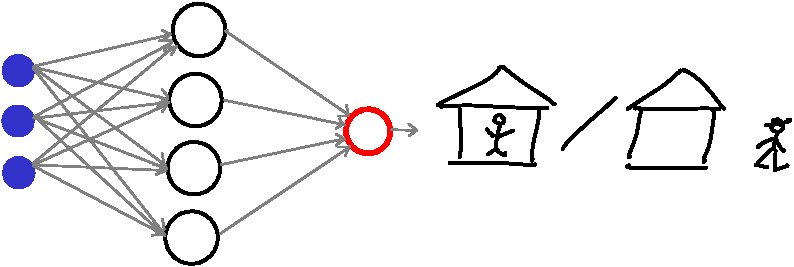
\includegraphics[width=0.6\textwidth]{neuralnet3-4-1-classif-crop.pdf}\\
\end{center}
\begin{itemize}
\item $e$ : entrées (ex. $e_1$ = longitude, $e_2$ = latitude, $e_3$ = température)
\item $t(e) \in \{0,1\}$ : fonction cible à apprendre ($t=1$ si la personne reste, $t=0$ sinon)
\item Ensemble de \alert{données} observées : $(e^i



%%%%%%%%%%%%%%%%%%%%%%%%%%%%%%%%%%%%%%%%%%%%%%%%%%%%%%%%%%%%%%%%%
\begin{frame}
\frametitle{Exemple d'optimisation : classification par RN (2/3)}
\begin{itemize}
\item $y(e;x)$ : Sortie du réseau de neurones $\in \mathbb R ~\ne~ \{0,1\}$ : l'espace de la fonction à apprendre est discret, celui du réseau est continu \Sadey[1.5][red!60!white]
\item Astuce : prédire la probabilité que $t(e)=1$. Cette probabilité est dans $[0,1]$ qui est continu... mais borné \Sey[1.5][red!30!white]
\item Astuce de la régression logistique : passer la sortie du RN dans une sigmoïde 
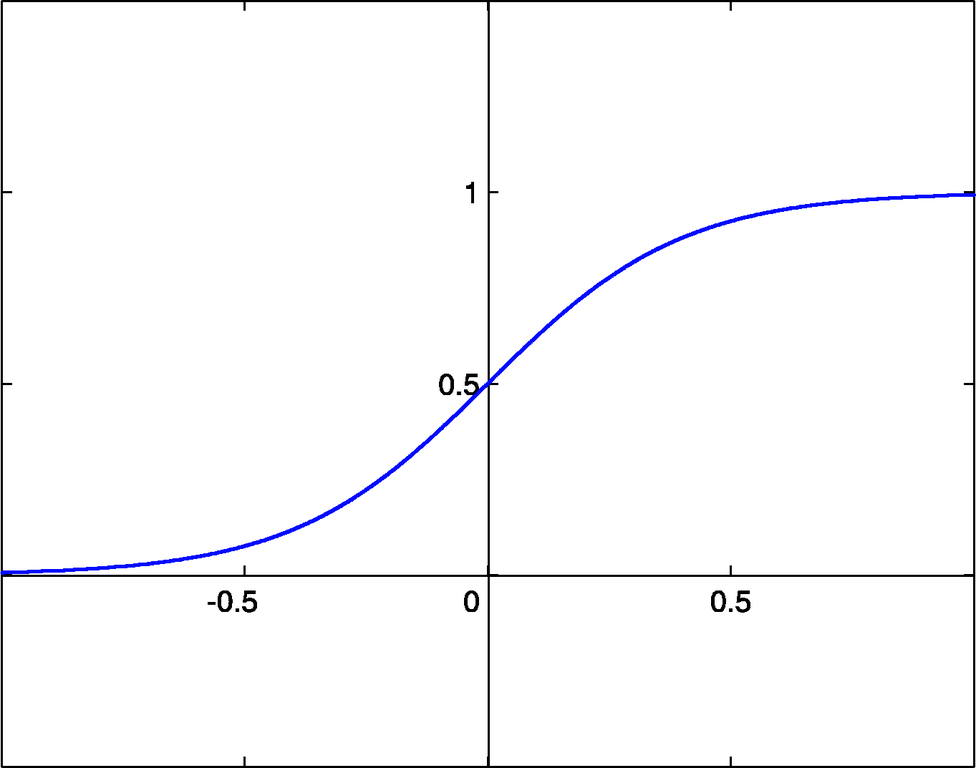
\includegraphics[width=0.16\textwidth]{SigmoidFunction.png}
pour obtenir $y(\cdot ; x) \in [0,1]$ \Tongey[1.5][green!60!white]
\item Avantage : le modèle a une interprétation probabiliste. $y(e;x)$ est la probabilité que $t(e)=1$, $t(e)$ est une variable de Bernoulli.
\end{itemize}
\end{frame}

%%%%%%%%%%%%%%%%%%%%%%%%%%%%%%%%%%%%%%%%%%%%%%%%%%%%%%%%%%%%%%%%%
\begin{frame}
\frametitle{Exemple d'optimisation : classification par RN (3/3)}
\alert{Erreur d'entropie croisée} comme distance modèle-données : 
\begin{equation*}
f(x) = - \sum_{i=1}^N \{ t^i \log(y(e^i;x)) + (1-t^i) \log(1 - y(e^i;x))\}
\end{equation*}
Démonstration :\\
\begin{itemize}
\item $y(e;x)$ est la probabilité que $t(e)=1$, $1-y(e;x)$ est la proba que $t(e)=0$, $0 \le y(e;x) \le 1$.
\item La probabilité de $t$ sachant $e$ peut s'écrire $y(e;x)^t \times (1 - y(e;x))^{1-t}$
\item La vraisemblance des $N$ observations i.i.d. est $\prod_{i=1}^N \left[y(e^i;x)^{t^i} \times (1-y(e^i;x))^{1-t^i}\right]$, à maximiser
\item On transforme la vraisemblance en erreur, à minimiser, en prenant $-\log(\text{vraisemblance})$ \qquad $\square$
\end{itemize}
\end{frame}

%%%%%%%%%%%%%%%%%%%%%%%%%%%%%%%%%%%%%%%%%%%%%%%%%%%%%%%%%%%%%%%%%
\begin{frame}
\begin{center}
{\usebeamercolor[fg]{title} 
\textbf{
Autres exemples d'utilisation de l'optimisation
} % end textbf
}% end color
\end{center}
\end{frame}

%%%%%%%%%%%%%%%%%%%%%%%%%%%%%%%%%%%%%%%%%%%%%%%%%%%%%%%%%%%%%%%%%
\begin{frame}
\frametitle{Exemple d'optimisation : conception}
\begin{center}
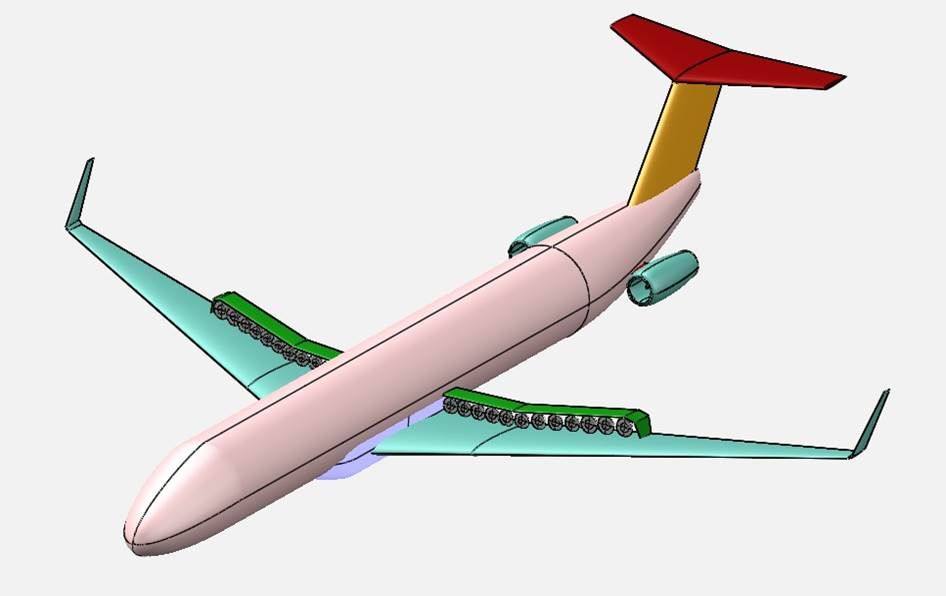
\includegraphics[width=0.5\textwidth]{aircraft_distributed_prop.png}\\
\vspace{-1cm}
{\hfill\tiny (tiré de \cite{sgueglia2018exploration})}
\end{center}
\vskip\baselineskip
$x$ = paramètres de l’avion (ici propulsion électrique distribuée)\\
$f()$ = $-1\times$ métrique de performance (agrégation de $-1\times$ portée, coût, distance de décollage, \ldots) \\
Au minimum, la conception est ``optimale''.
\end{frame}

%%%%%%%%%%%%%%%%%%%%%%%%%%%%%%%%%%%%%%%%%%%%%%%%%%%%%%%%%%%%%%%%%
\begin{frame}
\frametitle{Exemple d'optimisation : identification de modèle}
\begin{center}
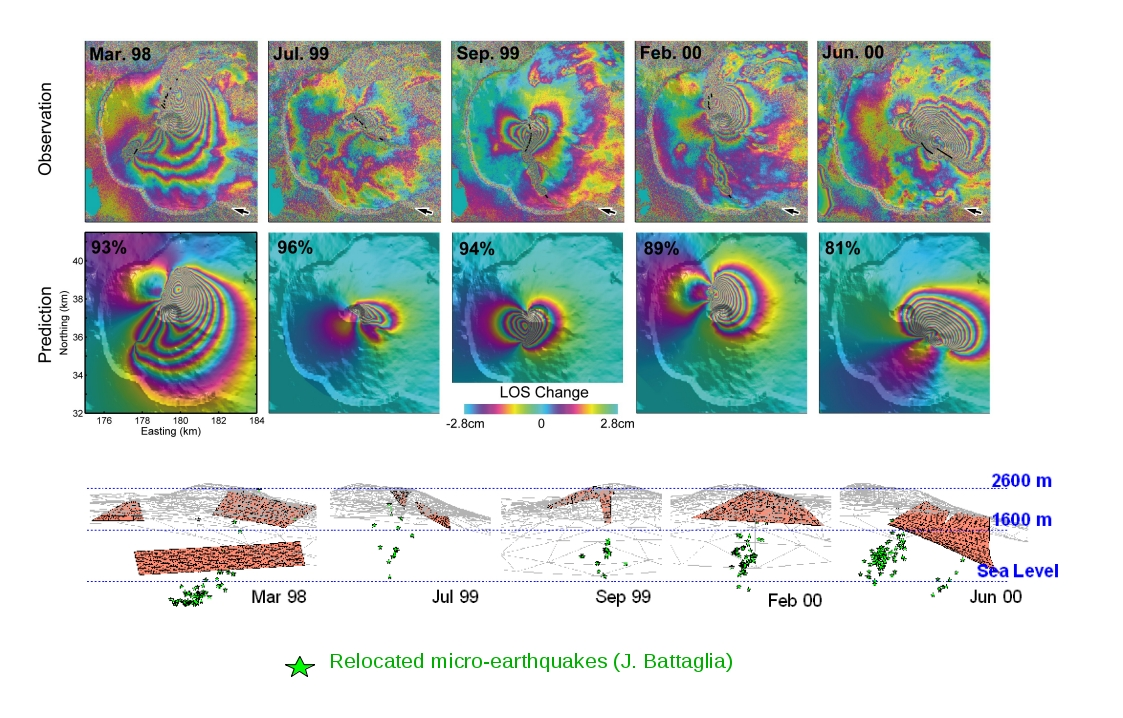
\includegraphics[width=0.7\textwidth]{piton_fournaise.jpg}\\
\vspace{-1cm}
{\hfill\tiny (tiré de \cite{fukushima2010evolution})}
\end{center}
$x$ = position du dyke, géométrie, pression interne\\
$f()$ = distance entre les mesures (du satellite RADARSAT-1) et le modèle (éléments de frontière, calcul non trivial)\\
Au minimum, le modèle correspond le mieux aux mesures et devrait représenter le phénomène souterrain.
\end{frame}

%%%%%%%%%%%%%%%%%%%%%%%%%%%%%%%%%%%%%%%%%%%%%%%%%%%%%%%%%%%%%%%%%
\begin{frame}
\frametitle{Exemple d'optimisation : débruitage d'image}
\vspace{-0.5cm}
\begin{equation*}
\begin{split}
\min_x f(x) \quad,\quad & f(x) = \frac{1}{2}\sum_{i=1}^{N_{\text{pixels}}} (y_i - x_i)^2 + 
\lambda \sum_{i=1}^{N_{\text{pixels}}} \sum_{j \text{ proche de } i} \lvert x_i - x_j \rvert \\
& \lambda \ge 0 \quad\text{constante de régularisation}
\end{split}
\end{equation*}
\begin{center}
\begin{minipage}[t]{0.2\textwidth}

\includegraphics[width=\textwidth]{c_clean.png} \\
{\small image cible}
\end{minipage}
\hfill
\begin{minipage}[t]{0.2\textwidth}
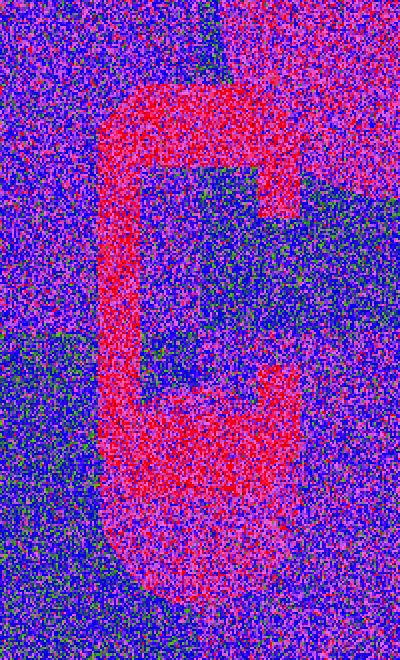
\includegraphics[width=\textwidth]{c_noisy.png} \\
{\small \mbox{bruitée (observée)} $= y_i$}
\end{minipage}
\hfill
\begin{minipage}[t]{0.2\textwidth}
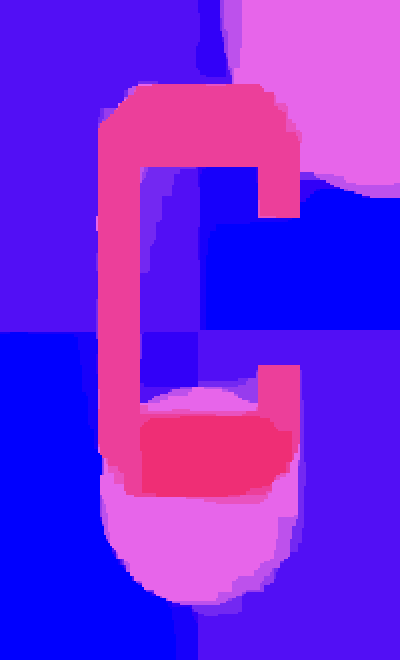
\includegraphics[width=\textwidth]{c_denoised.png} \\
{\small \mbox{dénoyautée (optimisée)} $=x^\star$}
\end{minipage}
\mbox{\quad}
\end{center}
{\scriptsize (tiré de \cite{ravikumar17}) \hfill}
\end{frame}


\subsection{Concepts mathématiques de base pour l'optimisation}

%%%%%%%%%%%%%%%%%%%%%%%%%%%%%%%%%%%%%%%%%%%%%%%%%%%%%%%%%%%%%%%%%%
\begin{frame}%[allowframebreaks]
\frametitle{Concepts mathématiques de base pour l'optimisation} 
\begin{multicols}{2}
\tableofcontents[currentsection]
\end{multicols}
\end{frame}

%%%%%%%%%%%%%%%%%%%%%%%%%%%%%%%%%%%%%%%%%%%%%%%%%%%%%%%%%%%%%%%%%%
\begin{frame}
\frametitle{Optimum local versus global} 
\vspace{-0.5cm}
\begin{equation*}
\min_{x \in \mathcal S \subset \Rset[n]} f(x)
\end{equation*}
\vspace{-0.5cm}
\begin{center}
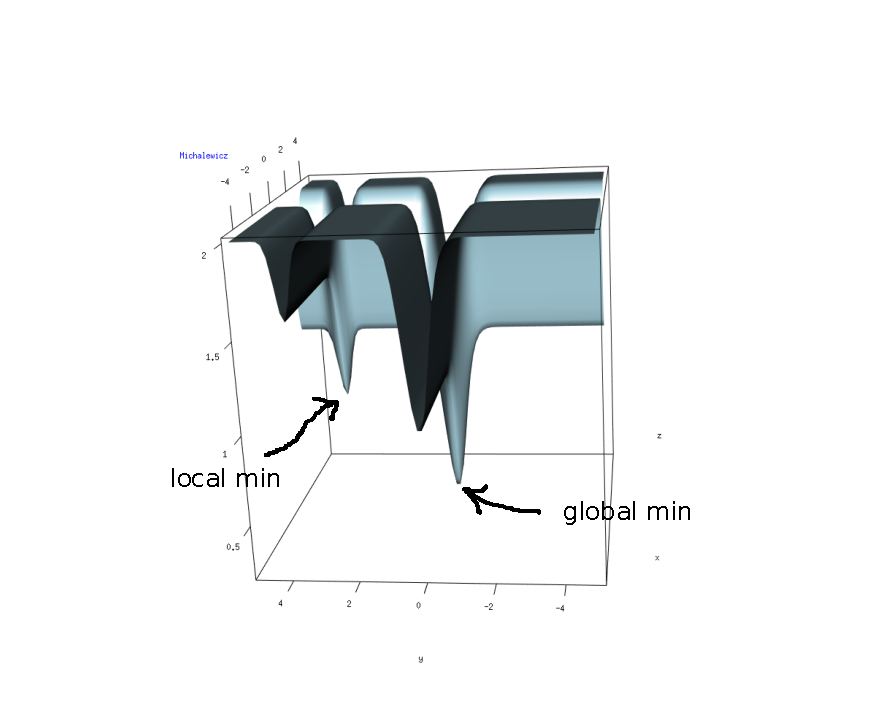
\includegraphics[width=0.7\textwidth]{michalewicz_function_annotated-crop.pdf} \\
\end{center}
\vspace{-1.0cm}
Code Python pour générer un tel graphique 3D disponible dans le dossier \texttt{Code}, fichier \texttt{3D\_plots.py} \\
\vfill
\end{frame}

%%%%%%%%%%%%%%%%%%%%%%%%%%%%%%%%%%%%%%%%%%%%%%%%%%%%%%%%%%%%%%%%%%
\begin{frame}
\frametitle{Gradient d'une fonction} 
Gradient d'une fonction = direction de la montée la plus rapide = vecteur des dérivées partielles
\begin{equation*}
\grad f(x) = \begin{pmatrix} \frac{\partial f}{\partial x_1}(x) \\ \ldots \\ \frac{\partial f}{\partial x_n}(x) \end{pmatrix}
\end{equation*}
\begin{center}
\begin{minipage}[t]{0.7\textwidth}
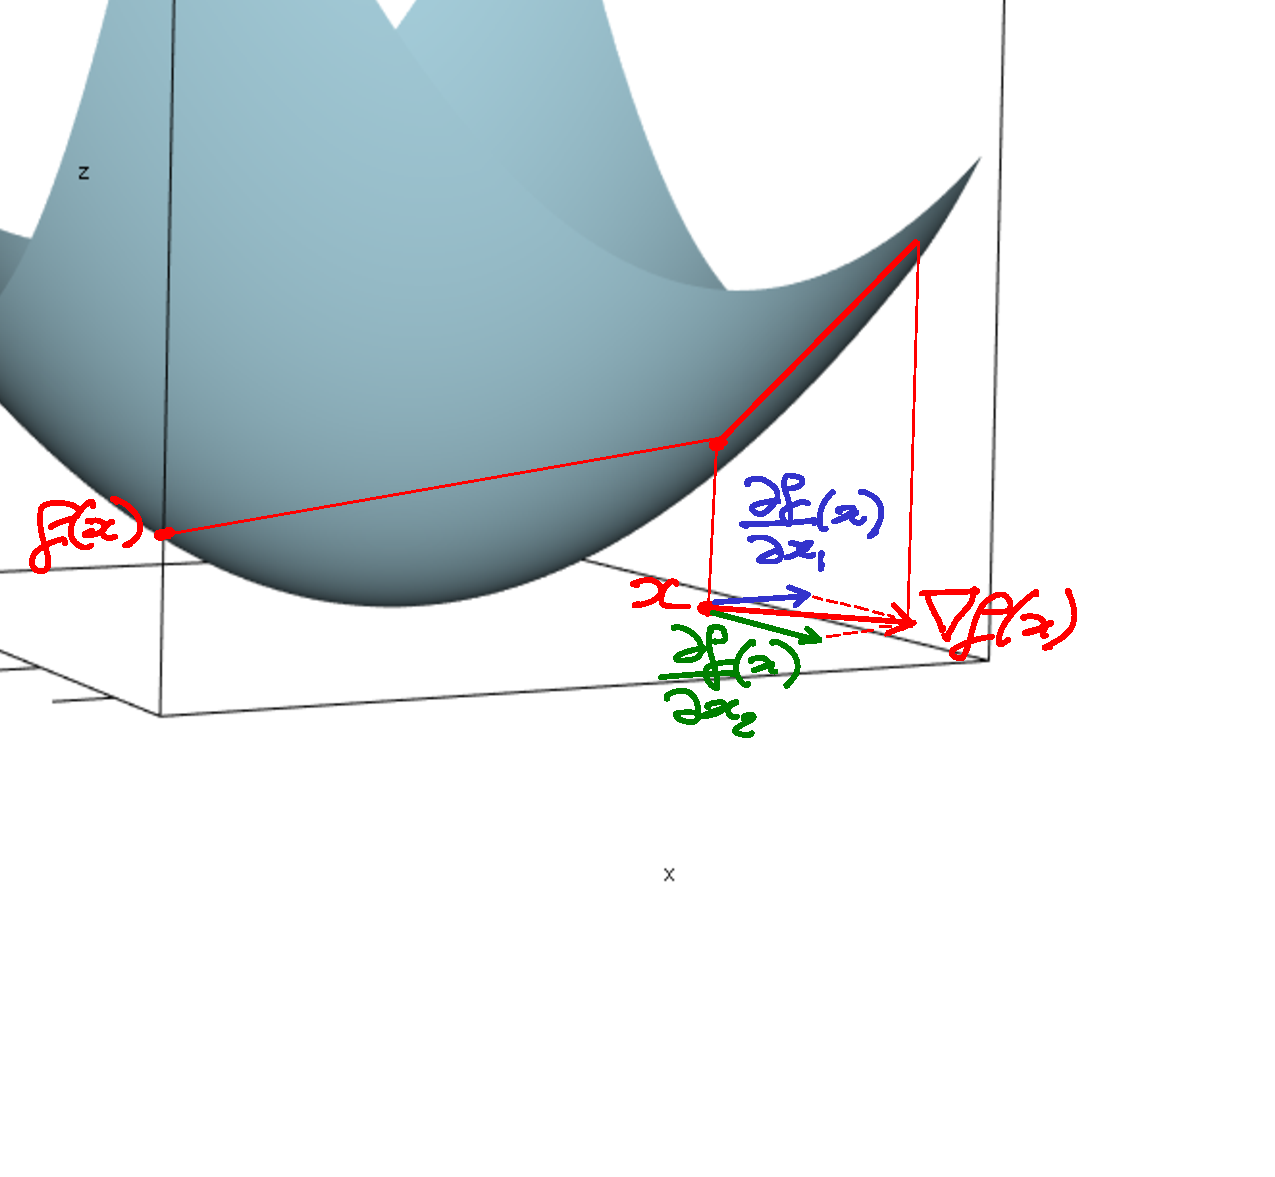
\includegraphics[width=\textwidth]{gradient-crop.pdf} \\
\end{minipage}
\end{center}
\end{frame}

%%%%%%%%%%%%%%%%%%%%%%%%%%%%%%%%%%%%%%%%%%%%%%%%%%%%%%%%%%%%%%%%%%
\begin{frame}
\frametitle{Hessienne d'une fonction} 
C’est la matrice des dérivées secondes,
\begin{equation*}
\hess f(x) = 
\begin{bmatrix}
\frac{\partial^2 f(x)}{\partial x_1^2} & \frac{\partial^2 f(x)}{\partial x_1 \partial x_2} & \ldots & \frac{\partial^2 f(x)}{\partial x_1 \partial x_n}\\ 
\frac{\partial^2 f(x)}{\partial x_1 \partial x_2} & \frac{\partial^2 f(x)}{\partial x_2^2} & \ldots & \frac{\partial^2 f(x)}{\partial x_2 \partial x_n}\\
\ldots & \ldots & \ddots & \ldots \\
\frac{\partial^2 f(x)}{\partial x_1 \partial x_n} & \frac{\partial^2 f(x)}{\partial x_2 \partial x_n} & \ldots & \frac{\partial^2 f(x)}{\partial x_n^2}
\end{bmatrix}
\end{equation*}
= matrice des courbures = gradient du gradient.
\end{frame}

%%%%%%%%%%%%%%%%%%%%%%%%%%%%%%%%%%%%%%%%%%%%%%%%%%%%%%%%%%%%%%%%%%
\begin{frame}[allowframebreaks]
\frametitle{Fonction quadratique et Hessienne} 
\vskip -0.5cm
\begin{equation*}
f(x) ~=~ \frac{1}{2} x^\top H x \quad , \quad \hess f(x) = H
\end{equation*}
une bonne approximation de ce qui se passe pour toute fonction au voisinage de la convergence
\mbox{
\begin{minipage}{0.5\textwidth}
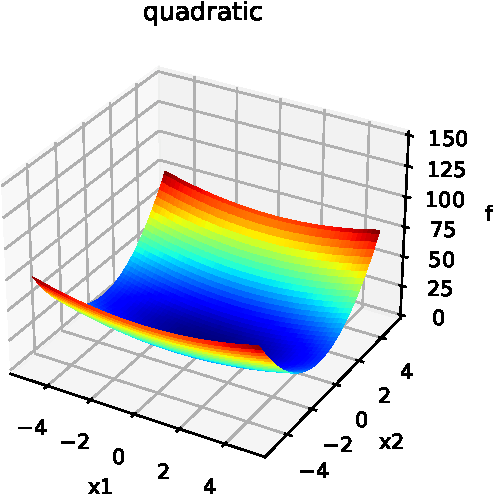
\includegraphics[width=\textwidth]{quad_rot0_cond5_H_1_0_0_5-crop.pdf}
\end{minipage}
\begin{minipage}{0.4\textwidth}
\begin{equation*}
H = \begin{bmatrix} 1 & 0 \\ 0 & 5\end{bmatrix}
\end{equation*}
\vskip\baselineskip
(devinez les valeurs propres et vecteurs propres)
\end{minipage}
}
%%%
\newpage
\begin{minipage}{0.5\textwidth}
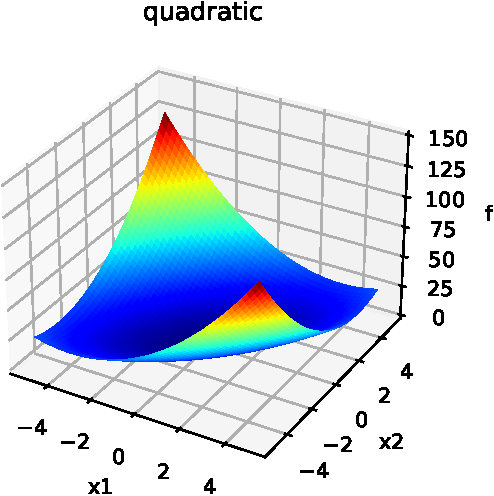
\includegraphics[width=\textwidth]{quad_rot45_cond5_H_3_m2_m2_3-crop.pdf}
\end{minipage}
\begin{minipage}{0.4\textwidth}
le même tourné de 45$^\circ$
\begin{align*}
H =& \begin{bmatrix} 3 & -2 \\ -2 & 3\end{bmatrix}  \\
\text{vect. propres} =& \begin{bmatrix} \sqrt{2}/2 & -\sqrt{2}/2 \\  \sqrt{2}/2 & \sqrt{2}/2 \end{bmatrix}\\
\text{val. propres} = & [1, 5]
\end{align*}
\end{minipage}
%%%
\newpage
\begin{minipage}{0.5\textwidth}
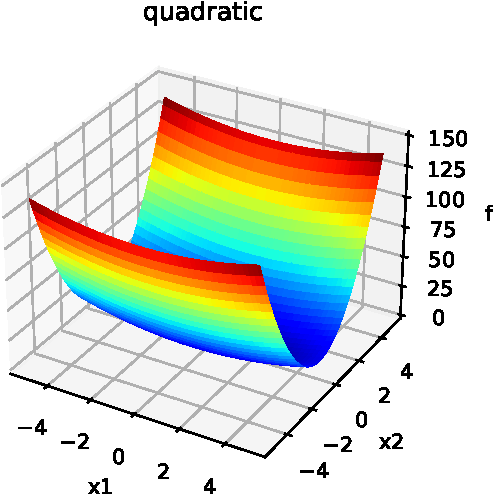
\includegraphics[width=\textwidth]{quad_rot0_cond10_H_1_0_0_10-crop.pdf}
\end{minipage}
\begin{minipage}{0.4\textwidth}
courbure accrue \\ 
(nombre de condition)
\begin{align*}
H =& \begin{bmatrix} 1 & 0 \\ 0 & 10\end{bmatrix}  
\end{align*}
\end{minipage}
%%%
\newpage
\begin{minipage}{0.5\textwidth}
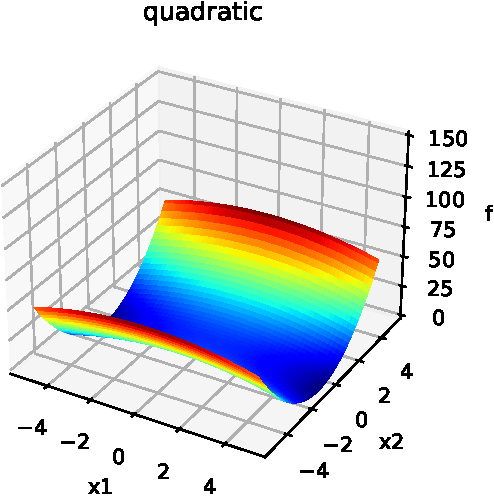
\includegraphics[width=\textwidth]{quad_rot0_condm5_H_m1_0_0_5-crop.pdf}
\end{minipage}
\begin{minipage}{0.4\textwidth}
Hessienne non définie positive
\begin{align*}
H =& \begin{bmatrix} -1 & 0 \\ 0 & 5\end{bmatrix}  
\end{align*}
quel est le problème ?
\end{minipage}
\end{frame}

%%%%%%%%%%%%%%%%%%%%%%%%%%%%%%%%%%%%%%%%%%%%%%%%%%%%%%%%%%%%%%%%%%
\begin{frame}
\frametitle{Approximation numérique du gradient} 
\mbox{
\begin{minipage}[b]{0.6\textwidth}
Par différences finies avant 
\begin{equation*}
\frac{\partial f(x)}{\partial x_i} \approx \frac{f(x+h e^i)-f(x)}{h}
\end{equation*}
{Démonstration : \scriptsize
par Taylor,\\
$f(x+he^i) = f(x) + h {e^i}^\top \cdot \nabla f(x) + \frac{h^2}{2} {e^i}^\top \mathrm{Hess} f(x+\rho h e^i) e^i, \quad \rho \in ]0,1[$ \\
$\frac{\partial f(x)}{\partial x_i} = \frac{f(x+he^i)-f(x)}{h} - \frac{h}{2} {e^i}^\top \mathrm{Hess} f(x+\rho h e^i) e^i$ \\
et en faisant tendre $h$ vers zéro $\square$
}
\end{minipage}
\begin{minipage}[b]{0.4\textwidth}
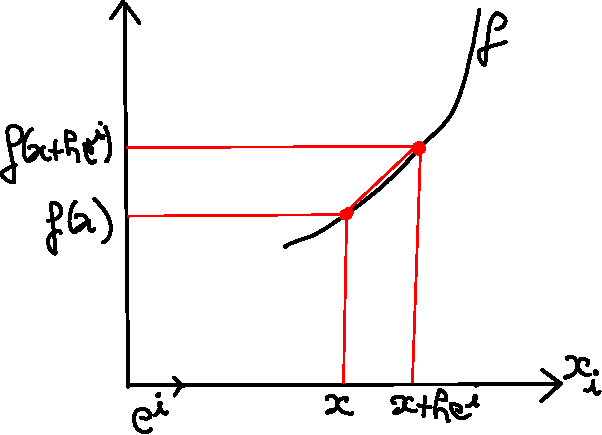
\includegraphics[width=\textwidth]{finitediff-crop.pdf}
\end{minipage}
} % mbox
\vskip\baselineskip
Autres schémas (meilleurs mais plus complexes à implémenter) : différences centrées, différentiation automatique (ex. : TensorFlow ou PyTorch), différentiation (semi-)analytique (ex. : rétropropagation dans les réseaux de neurones).
\end{frame}

%%%%%%%%%%%%%%%%%%%%%%%%%%%%%%%%%%%%%%%%%%%%%%%%%%%%%%%%%%%%%%%%%%
\begin{frame}
\frametitle{Direction de descente} 
\mbox{
\begin{minipage}[b]{0.5\textwidth}
Une direction de recherche $d$ formant un angle aigu avec $-\nabla f(x)$ est une direction de descente, c’est-à-dire que pour un pas suffisamment petit, $f$ diminue assurément !
\end{minipage}
\hfill
\begin{minipage}[t]{0.4\textwidth}
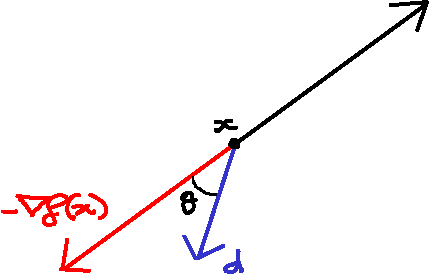
\includegraphics[width=\textwidth]{descent_direction-crop.pdf}
\end{minipage}
}
\\\vspace{0.8cm}
{\normalsize
Démonstration : par Taylor, $\forall \alpha,~\exists \epsilon \in [0,1]$ tel que
$f(x+\alpha d) = f(x) + \alpha d^\top \cdot \nabla f(x) + \frac{\alpha^2}{2} d^\top \mathrm{Hess} f(x + \alpha \epsilon d) d$\\
$\lim_{\alpha \rightarrow 0^+} \frac{f(x+\alpha d) - f(x)}{\alpha} = d^\top \cdot \nabla f(x) = - 1 \times \lVert \nabla f(x) \rVert \cos(d,-\nabla f(x))$ \\
est négatif si le cosinus est positif $\square$
}
\end{frame}

%%%%%%%%%%%%%%%%%%%%%%%%%%%%%%%%%%%%%%%%%%%%%%%%%%%%%%%%%%%%%%%%%%
\begin{frame}
\frametitle{Condition nécessaire d’optimalité (1)} 
Une condition nécessaire pour qu’une fonction différentiable ait un minimum en $x^\star$ est que celle-ci soit plate en ce point, c’est-à-dire que son gradient soit nul :
\begin{equation*}
x^\star \in \arg \min_{x \in \mathcal S} f(x) \Rightarrow \nabla f(x^\star) = 0
\end{equation*}
\vskip\baselineskip
\begin{center}
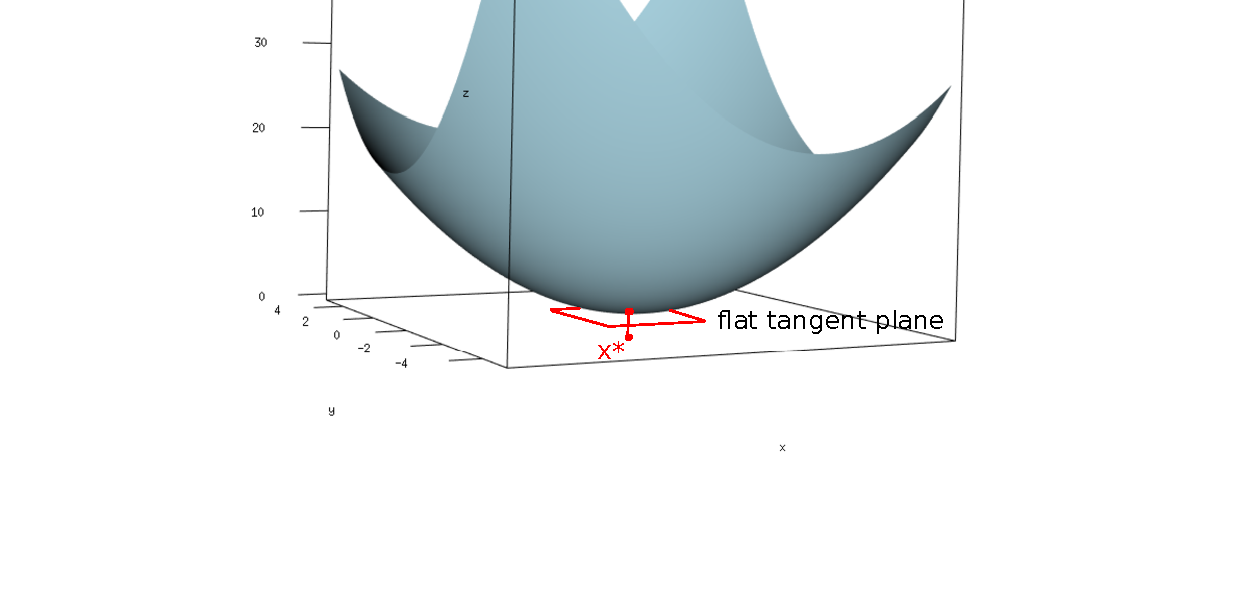
\includegraphics[width=1.2\textwidth]{minimum-crop.pdf} \\
\end{center}
\end{frame}

%%%%%%%%%%%%%%%%%%%%%%%%%%%%%%%%%%%%%%%%%%%%%%%%%%%%%%%%%%%%%%%%%%
\begin{frame}
\frametitle{Condition nécessaire d’optimalité (2)} 
\begin{center}
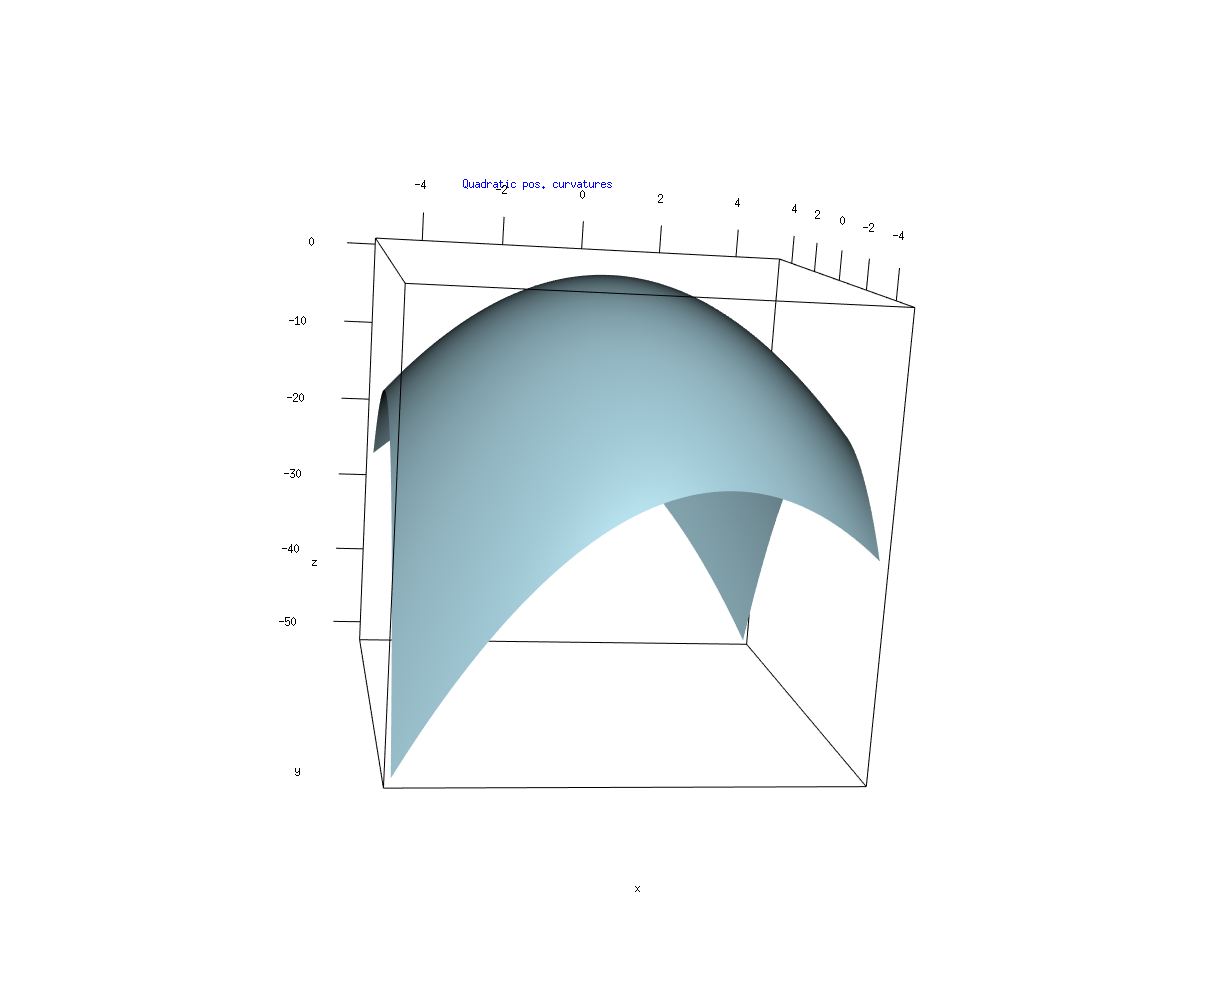
\includegraphics[width=0.7\textwidth]{quad_neg_curv.png} \\
nécessaire mais pas suffisante (fonctionne aussi pour un maximum) 
\vspace{2cm}
\end{center}
\end{frame}

%%%%%%%%%%%%%%%%%%%%%%%%%%%%%%%%%%%%%%%%%%%%%%%%%%%%%%%%%%%%%%%%%%
\begin{frame}
\frametitle{Condition nécessaire d’optimalité (3)} 
\begin{center}
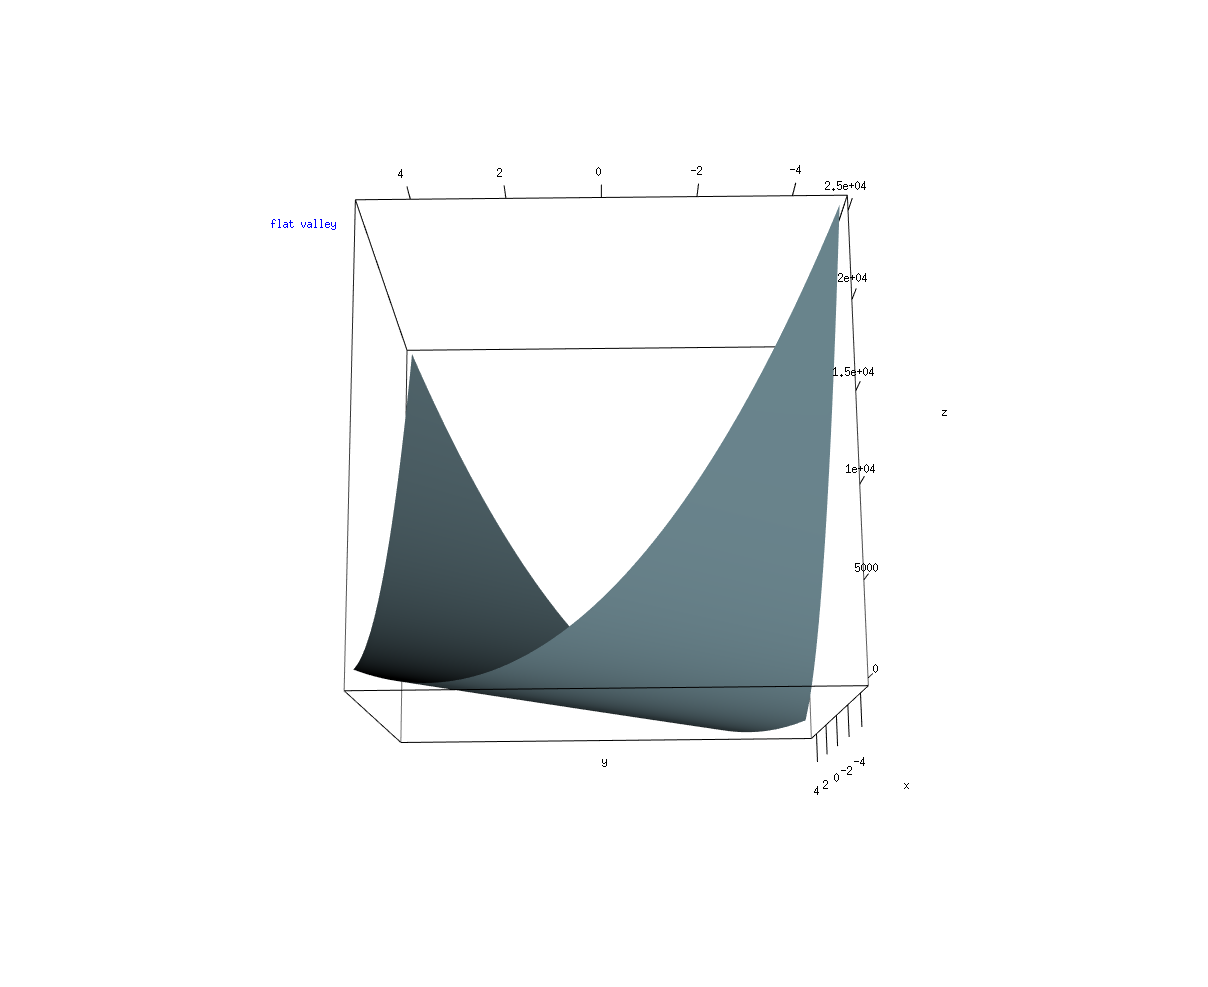
\includegraphics[width=0.7\textwidth]{flat_valley.png} \\
$\nabla f(x^\star) = 0$ ne garantit pas l’unicité de $x^\star$ (vallée plate)
\end{center}
\end{frame}

%%%%%%%%%%%%%%%%%%%%%%%%%%%%%%%%%%%%%%%%%%%%%%%%%%%%%%%%%%%%%%%%%%
\begin{frame}
\frametitle{Condition nécessaire d’optimalité (4)} 
\begin{center}
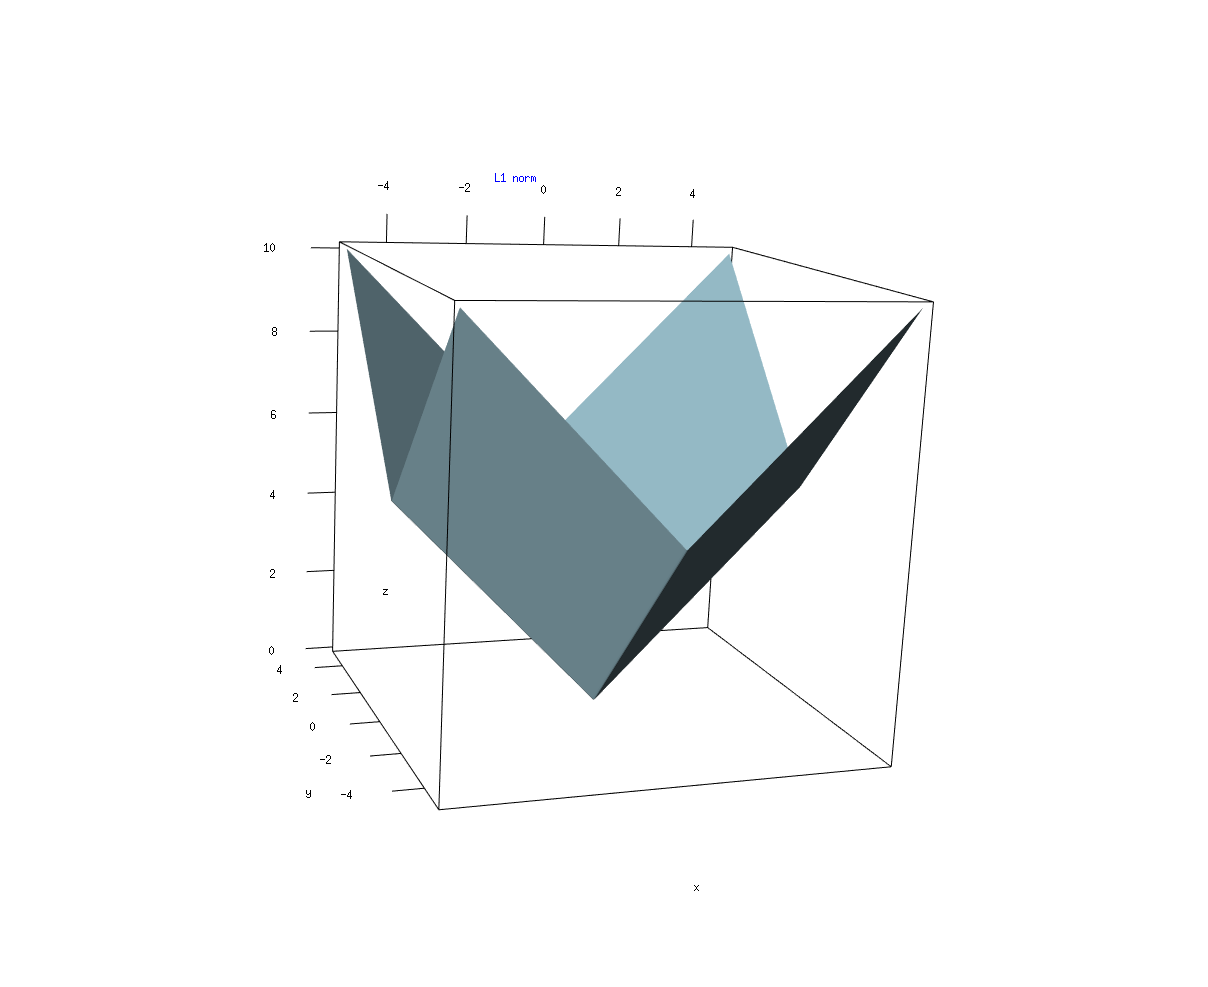
\includegraphics[width=0.7\textwidth]{L1norm.png} \\
$\nabla f()$ n’est pas défini partout, exemple avec la norme L1 $= \sum_{i=1}^n |x_i|$
\end{center}
\end{frame}


\section{Algorithme de la descente la plus raide}

%%%%%%%%%%%%%%%%%%%%%%%%%%%%%%%%%%%%%%%%%%%%%%%%%%%%%%%%%%%%%%%%%%
\begin{frame}%[allowframebreaks]
\frametitle{Plan du cours} 
\begin{multicols}{2}
\begin{center} \textbf{Introduction à l’optimisation pour l’apprentissage automatique} \end{center}
\tableofcontents[currentsection]
\end{multicols}
\end{frame}


%%%%%%%%%%%%%%%%%%%%%%%%%%%%%%%%%%%%%%%%%%%%%%%%%%%%%%%%%%%%%%%%%%
\begin{frame}
\frametitle{Optimiseurs comme algorithmes itératifs} 
\begin{equation*}
\text{On cherche } \quad  x^\star \in \arg\min_{x \in \mathcal S} f(x) \quad,\quad \mathcal S = \mathbb{R}^n
\end{equation*}
\begin{itemize}
\item Sauf cas particuliers (ex. : problèmes quadratiques convexes), la solution n’est pas obtenue analytiquement via les conditions d’optimalité ($\nabla f(x^\star) = 0$ + conditions d’ordre supérieur).
\item On utilise typiquement des algorithmes itératifs : $x^{i+1}$ dépend des itérés précédents $x^1, \ldots, x^i$ et de leurs valeurs $f$.
\item Souvent, calculer $f(x^i)$ demande plus de temps que l’algorithme d’optimisation lui-même.
\item Qualités recherchées chez un optimiseurs : robustesse, rapidité de convergence. Il faut un compromis entre ces deux.
\end{itemize}
\end{frame}

\subsection{Algorithme de la descente la plus raide à pas fixe}

%%%%%%%%%%%%%%%%%%%%%%%%%%%%%%%%%%%%%%%%%%%%%%%%%%%%%%%%%%%%%%%%%%
\begin{frame}
\frametitle{Algorithme de la descente la plus raide à pas fixe (1)} 
Répéter les étapes dans la direction de la descente la plus raide, $-\nabla f(x^t)$ \cite{cauchy1847methode,curry1944method}. \\
La taille des pas est proportionnelle à la norme du gradient.
\begin{block}{}
\begin{algorithmic}
\REQUIRE $f()$, $\bar\alpha \in ]0,1]$, $x^1$, $\epsilon^{\text{step}}$, $\epsilon^{\text{grad}}$, $i^{\text{max}}$
\STATE $i \leftarrow 0$, $f^{\text{bestSoFar}} \leftarrow$ \texttt{max\_double}
\REPEAT 
\STATE $i \leftarrow i+1$
\STATE calculer $f(x^i)$ et $\nabla f(x^i)$
\IF{$f(x^i) < f^{\text{bestSoFar}}$} 
\STATE mettre à jour $x^{\text{bestSoFar}}$ et $f^{\text{bestSoFar}}$ avec l’itéré courant
\ENDIF
\STATE \textbf{direction : } $d^i = - \frac{\nabla f(x^i)}{\lVert \nabla f(x^i) \rVert}$
\STATE \textbf{pas : } $x^{i+1} = x^i + \bar\alpha \lVert \nabla f(x^i) \rVert d^i$
\UNTIL{ {$i > i^{\text{max}}$} \OR {$\lVert x^i - x^{i-1} \rVert \le \epsilon^{\text{step}}$} \OR {$\frac{\lVert \nabla f(x^i) \rVert}{\sqrt{n}} \le \epsilon^{\text{grad}}$} }
\RETURN $x^{\text{bestSoFar}}$ et $f^{\text{bestSoFar}}$
\end{algorithmic}
\end{block}
\end{frame}




%%%%%%%%%%%%%%%%%%%%%%%%%%%%%%%%%%%%%%%%%%%%%%%%%%%%%%%%%%%%%%%%%%
\begin{frame}
\frametitle{(organisation du code)}
\vspace{-0.4cm}
\begin{itemize}
\small
\item Dans \texttt{src/optimcourse} : fichiers ressources pour l’optimisation
\begin{itemize}
\small
\item \texttt{gradient_descent.py}, \texttt{restarted_gradient_descent.py} : algorithmes de descente basés sur le gradient ; la version actuelle à pas fixe, et celles à venir (autre direction, avec recherche linéaire), une version avec recherches aléatoires relancées.
\item \texttt{random_search.py} : un algorithme de recherche aléatoire.
\item \texttt{test_functions.py} : une collection de fonctions tests.
\item \texttt{3D_plots.py} : trace une fonction bidimensionnelle en 3D + tracé des contours.
\item \texttt{optim_utilities.py} : routines additionnelles.
\end{itemize}
\item Dans \texttt{src/optimcourse} : fichiers ressources pour le réseau de neurones codé de zéro
\begin{itemize}
\small
\item \texttt{activation_functions.py} : la collection des fonctions d’activation.
\item \texttt{forward_propagation.py} : collection de routines pour la propagation avant dans un réseau de neurones.
\end{itemize}
\item Dans \texttt{notebooks} : notebooks et script principal pour lancer les algorithmes de descente et entraîner les réseaux de neurones.
\end{itemize}
\end{frame}
%%%%%%%%%%%%%%%%%%%%%%%%%%%%%%%%%%%%%%%%%%%%%%%%%%%%%%%%%%%%%%%%%%
\begin{frame}
\frametitle{Algorithme de descente du gradient à pas fixe (2)}
\begin{itemize}
\item Le choix du facteur de taille de pas $\bar\alpha$ est critique : plus la fonction est raide, plus $\bar\alpha$ doit être petit. Valeur par défaut = 0.1
\item Le vrai code (cf. \texttt{gradient_descent.R}) est un peu plus long car il faut enregistrer les points visités.
\end{itemize}
\vspace{-0.5cm}
\begin{center}
{\scriptsize $f(x) = \frac{1}{2} x^\top H x$ , $H$ définie positive}\
\begin{minipage}[b]{0.3\textwidth}
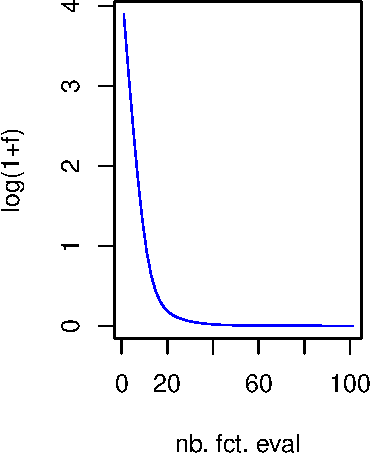
\includegraphics[width=\textwidth]{gradient_quad_2d_f_alpha01-crop.pdf}
\end{minipage}
\hspace{1.5cm}
\begin{minipage}[b]{0.3\textwidth}
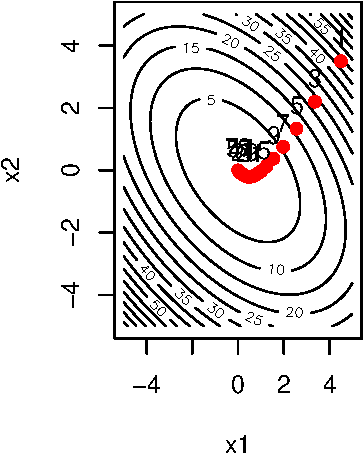
\includegraphics[width=\textwidth]{gradient_quad_2d_x_alpha01-crop.pdf}
\end{minipage}
\end{center}
\end{frame}
%%%%%%%%%%%%%%%%%%%%%%%%%%%%%%%%%%%%%%%%%%%%%%%%%%%%%%%%%%%%%%%%%%
\begin{frame}
\frametitle{Algorithme de descente du gradient à pas fixe (3)}
$\bar\alpha=0.1$ sur la fonction de Rosenbrock (en forme de banane) en dimension $d=2$, exemple de divergence :
\vskip\baselineskip
\begin{center}
\begin{minipage}[b]{0.3\textwidth}
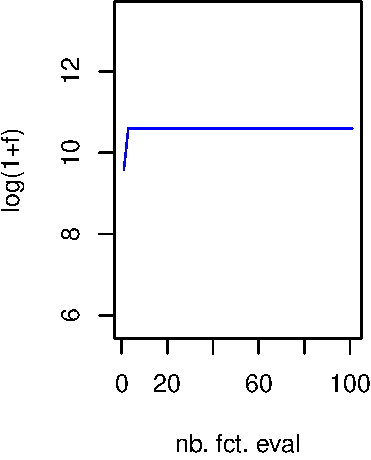
\includegraphics[width=\textwidth]{gradient_rosen_alpha0.1_f_diverges-crop.pdf}
\end{minipage}
\hspace{1.5cm}
\begin{minipage}[b]{0.3\textwidth}
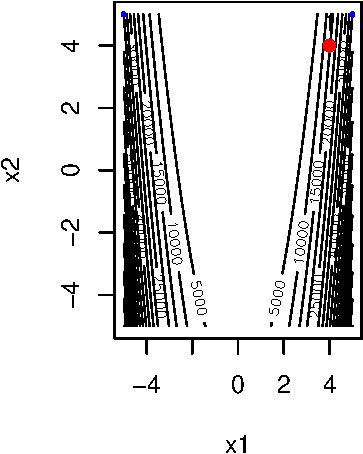
\includegraphics[width=\textwidth]{gradient_rosen_alpha0.1_x_diverges-crop.pdf}
\end{minipage}
$x^\star = (1,1) , f(x^\star) = 0$
\end{center}
\end{frame}
\subsection{Recherche linéaire}
%%%%%%%%%%%%%%%%%%%%%%%%%%%%%%%%%%%%%%%%%%%%%%%%%%%%%%%%%%%%%%%%%%
\begin{frame}
\frametitle{Descente avec recherche linéaire}
\vspace{-0.5cm}
À chaque itération, on cherche la meilleure taille de pas dans la direction de descente\footnote{si $d^i$ n’est pas une direction de descente, $-d^i$ l’est. Preuve laissée en exercice.} $d^i$ (qui pour l’instant est $-\grad f(x^i)/\lVert \grad f(x^i) \rVert$ mais peut être générale).\
Même algorithme que précédemment, on change juste l’instruction \textbf{pas} :
\begin{block}{}
\begin{algorithmic}
\REQUIRE \ldots
\STATE initialisations mais plus de $\alpha$ pour l’instant \ldots
\REPEAT
\STATE incrémenter $i$, calculer $f(x^i)$ et $\grad f(x^i)$ \ldots
\STATE \textbf{direction : } $d^i = - \grad f(x^i) / \lVert \grad f(x^i) \rVert$ ou toute autre \textbf{direction de descente}
\STATE \textbf{pas : } \textcolor{red}{$\alpha^{i} = \arg \min_{\alpha > 0} f(x^i+\alpha d^i)$ \
\hspace{1.5cm}$x^{i+1} = x^i + \alpha^i d^i$
} % fin rouge
\UNTIL critères d’arrêt
\RETURN meilleur résultat obtenu
\end{algorithmic}
\end{block}
\end{frame}
%%%%%%%%%%%%%%%%%%%%%%%%%%%%%%%%%%%%%%%%%%%%%%%%%%%%%%%%%%%%%%%%%%
\begin{frame}
\frametitle{Recherche linéaire approximative (1)}
Notation : pendant la recherche linéaire $i$,
\begin{eqnarray*}
x &=& x^i + \alpha d^i \
f(\alpha) &=& f(x^i + \alpha d^i) \
\frac{df(0)}{d\alpha} &=& \sum_{j=1}^n \frac{\partial f(x^i)}{\partial x_j} \frac{\partial x_j}{\partial \alpha}
=\sum_{j=1}^n \frac{\partial f(x^i)}{\partial x_j} d^i_j
= \grad f(x^i)^\top . d^i
\end{eqnarray*}
En pratique, optimiser parfaitement $\alpha^i$ est trop coûteux et inutile
$\Rightarrow$ on approxime la recherche linéaire par une condition de décroissance suffisante :
\begin{equation*}
\text{trouver } \alpha^i \text{ tel que } f(x^i + \alpha^i d^i) < f(x^i) + \delta \alpha^i \grad f(x^i)^\top . d^i
\end{equation*}
où $\delta \in [0,1]$, c’est-à-dire réaliser une proportion $\delta$ du progrès promis par le développement de Taylor d’ordre 1.
\end{frame}
%%%%%%%%%%%%%%%%%%%%%%%%%%%%%%%%%%%%%%%%%%%%%%%%%%%%%%%%%%%%%%%%%%
\begin{frame}
\frametitle{Recherche linéaire approximative (2)}
Condition de décroissance suffisante réécrite avec la notation de recherche linéaire :
\begin{equation*}
\text{trouver } \alpha^i \text{ tel que } f(\alpha^i) < f(x^i) + \delta \alpha^i \frac{d f(0)}{d \alpha}
\end{equation*}
\centering
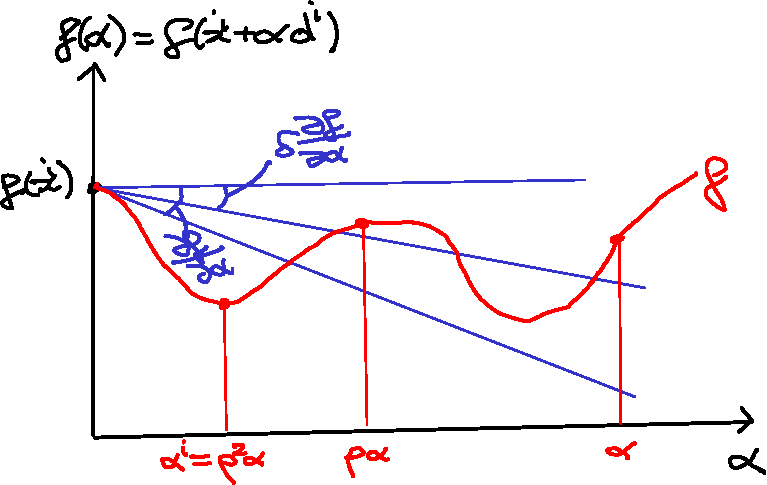
\includegraphics[width=0.7\textwidth]{line_search_backtrack-crop.pdf}
\end{frame}
%%%%%%%%%%%%%%%%%%%%%%%%%%%%%%%%%%%%%%%%%%%%%%%%%%%%%%%%%%%%%%%%%%
\begin{frame}
\frametitle{Recherche linéaire approximative (3)}
À l’itération $i$ :
\begin{block}{Recherche linéaire par retour en arrière (Armijo)}
\begin{algorithmic}
\REQUIRE $d^i$ une direction de descente, $x^i$, $\delta \in [0,1]$, $\rho \in ]0,1[$, $C>0$
\STATE (valeurs par défaut : $\delta=0.1,~\rho=0.5,~C=1$)
\STATE initialiser la taille de pas : $\alpha = \max(C \times \lVert \grad f(x^i) \rVert , \sqrt{n}/100) $
\WHILE{$f(x^i + \alpha d^i) \ge f(x^i) + \delta \alpha \grad f(x^i)^\top d^i$}
\STATE réduire la taille de pas : $\alpha \leftarrow \rho \times \alpha$
\ENDWHILE
\RETURN $\alpha^i \leftarrow \alpha$
\end{algorithmic}
\end{block}
Désormais, on utilise la recherche linéaire, et le nombre d’appels à $f$ n’est plus égal au nombre d’itérations car plusieurs appels à la fonction peuvent avoir lieu lors d’une recherche linéaire à l’intérieur d’une seule itération.
\end{frame}





%%%%%%%%%%%%%%%%%%%%%%%%%%%%%%%%%%%%%%%%%%%%%%%%%%%%%%%%%%%%%%%%%%
\begin{frame}
\frametitle{Recherche linéaire approximative (4)}
Regardons ce que fait la recherche linéaire sur $f(x)=$ fonction de Rosenbrock où le pas fixe a divergé
\begin{center}
\begin{minipage}[b]{0.3\textwidth}
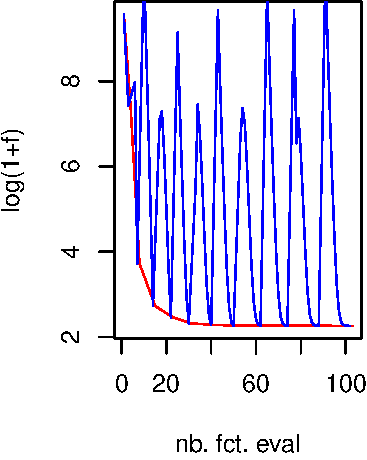
\includegraphics[width=\textwidth]{gradient_rosen_LS_f-crop.pdf}
\end{minipage}
\hspace{1.cm}
\begin{minipage}[b]{0.3\textwidth}
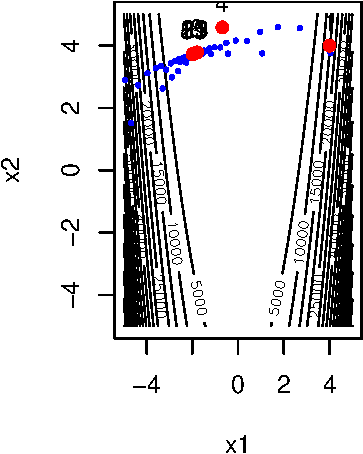
\includegraphics[width=\textwidth]{gradient_rosen_LS_x-crop.pdf}
\end{minipage}
\end{center}
Mieux, mais pas parfait : les oscillations ralentissent fortement les progrès.
\end{frame}
%%%%%%%%%%%%%%%%%%%%%%%%%%%%%%%%%%%%%%%%%%%%%%%%%%%%%%%%%%%%%%%%%
\begin{frame}
\frametitle{Vitesse de convergence du gradient}
$f(x) = \frac{1}{2} x^\top H x$ en dimension $n=10$, $H>0$, non alignée avec les axes, nombre de condition = 10.
\begin{center}
\mbox{
\begin{minipage}[c]{0.37\textwidth}
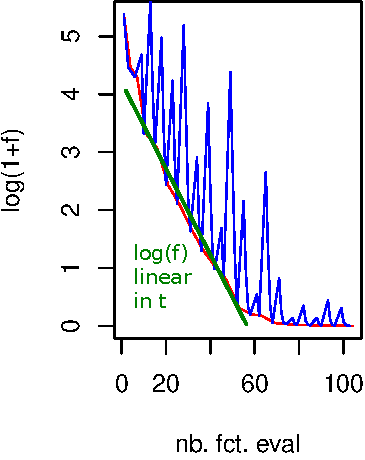
\includegraphics[width=\textwidth,height=6cm]{gradient_quad_d10_cond10_LS-lin-crop.pdf}
\end{minipage}
\hspace{0.5cm}
\begin{minipage}[c]{0.57\textwidth}
Empiriquement (pour les démonstrations et plus d'infos cf. \cite{ravikumar17}) : sur des fonctions convexes et différentiables, la recherche par gradient avec recherche linéaire progresse à une vitesse telle que
$f(x^t) \propto \xi \gamma^t$ où $\gamma \in [0,1[$.
Équivalent à dire que pour atteindre $f(x^t) < \varepsilon$, il faut $t > \mathcal{O}(\log(1/\varepsilon))$
\vskip\baselineskip
{\scriptsize
$\log f(x^t) \propto t \log(\gamma) + \log(\xi) \Rightarrow \log(\gamma) < 0$ pente de la courbe verte.\
$\xi \gamma^t < \varepsilon \Leftrightarrow t > \frac{\log(\varepsilon) - \log(\xi)}{\log(\gamma)} = \frac{-1}{\log(\gamma)} \log(\xi/\varepsilon)$\
$\Rightarrow~ t > \mathcal{O}(\log(1/\varepsilon))$.
} % fin scriptsize
\end{minipage}
} % fin mbox
\end{center}
\end{frame}
%%%%%%%%%%%%%%%%%%%%%%%%%%%%%%%%%%%%%%%%%%%%%%%%%%%%%%%%%%%%%%%%%%
\begin{frame}
\frametitle{Oscillations en descente de gradient}
La recherche linéaire parfaite résout
\begin{equation*}
\alpha^i = \arg\min_{\alpha>0} f(\alpha) \text{ où } f(\alpha) = f(x^i+\alpha d^i)
\end{equation*}
Conditions nécessaires pour la taille de pas optimale :
\begin{equation*}
\frac{df(\alpha^i)}{d\alpha} = \sum_{j=1}^n \frac{\partial f(x^i + \alpha^i d^i)}{\partial x_j} \frac{\partial x_j}{\partial \alpha}
= \grad f(x^{i+1})^\top \cdot d^i = 0
\end{equation*}
Si la direction est le gradient,
\begin{equation*}
{-d^{i+1}}^\top \cdot d^i = 0 ~\text{ c’est-à-dire } d^{i+1} \text{ et } d^i \text{ sont perpendiculaires}
\end{equation*}
\begin{center}
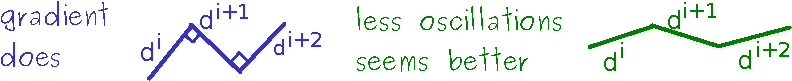
\includegraphics[width=\textwidth]{oscillations-crop.pdf}
\end{center}
\end{frame}
\section{Recherches améliorées basées sur le gradient}
%%%%%%%%%%%%%%%%%%%%%%%%%%%%%%%%%%%%%%%%%%%%%%%%%%%%%%%%%%%%%%%%%%
\begin{frame}
\frametitle{Plan du cours}
\begin{multicols}{2}
\begin{center} \textbf{Une introduction à l’optimisation pour l’apprentissage automatique} \end{center}
\tableofcontents[currentsection]
\end{multicols}
\end{frame}
\subsection{Directions de recherche pour accélération}
%%%%%%%%%%%%%%%%%%%%%%%%%%%%%%%%%%%%%%%%%%%%%%%%%%%%%%%%%%%%%%%%%%%
%\begin{frame}
%\frametitle{Gradient avec momentum (1)}
%Rappel de la descente de gradient à pas fixe,
%\begin{equation*}
%%x^{i+1} = x^i + \alpha s^i \quad\text{ où }\quad s^i= -\grad f(x^i)
%x^{i+1}= x^i - \bar\alpha \grad f(x^i) \quad\text{ c’est-à-dire } s^i = x^{i+1}-x^i = - \bar\alpha \grad f(x^i)
%\end{equation*}
%$s^i$, le pas, éventuellement corrigé par une recherche linéaire ($x^{i+1}= x^i + \alpha^i s^i/\lVert s^i \rVert$).
%Introduisons un momentum (une mémoire) dans le pas de recherche \cite{polyak1964some},
%\begin{equation*}
%s^i = -\bar\alpha\grad f(x^i) + \beta (x^i -x^{i-1})
%\end{equation*}
%où\footnote{alternativement, pour un momentum variable selon l’itération, $\beta^i=(i-2)/(i+1)$} $\beta = 0.9$.\
%\vspace{-0.2cm}
%\begin{minipage}[c]{0.5\textwidth}
%Cela devrait aider à éviter les oscillations qui surviennent au fond des vallées.\
%$s^i$ reste une direction de descente (en supposant une recherche linéaire parfaite).
%\end{minipage}
%\begin{minipage}[c]{0.4\textwidth}
%\begin{center}
%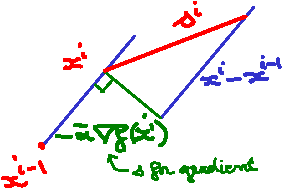
\includegraphics[width=0.9\textwidth]{momentum-crop.pdf}
%\end{center}
%\end{minipage}
%\end{frame}







%%%%%%%%%%%%%%%%%%%%%%%%%%%%%%%%%%%%%%%%%%%%%%%%%%%%%%%%%%%%%%%%%%%
%\begin{frame}
%\frametitle{Gradient avec momentum (2)}
%%Retour à Rosenbrock, $d=2$, $x^\star = (1,1) , f(x^\star) = 0$,\
%%budget=4000, $x^1=(4,4)$
%%\vspace{-0.3cm}
%%\begin{center}
%%\begin{minipage}[c]{0.35\textwidth}
%%\begin{center}
%%gradient\
%%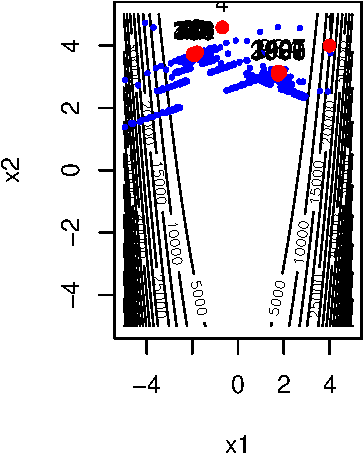
\includegraphics[width=\textwidth]{gradient_rosen_LS_budg4000_x-crop.pdf}
%%\end{center}
%%\end{minipage}
%%\begin{minipage}[c]{0.35\textwidth}
%%\begin{center}
%%momentum\
%%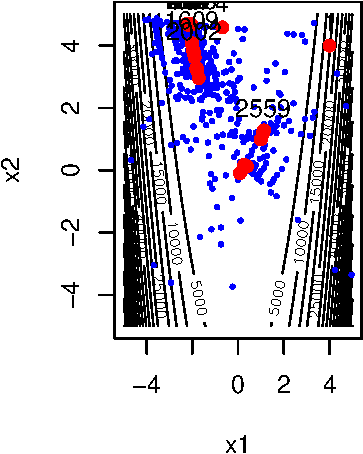
\includegraphics[width=\textwidth]{momentum_rosen_LS_budg4000_x-crop.pdf}
%%\end{center}
%%\end{minipage}
%%\end{center}
%%L'accélération par momentum permet de trouver la solution.
%Fonction quadratique, 10 dimensions, nombre de condition = 300, départ depuis [4,\ldots,4]
%\begin{center}
%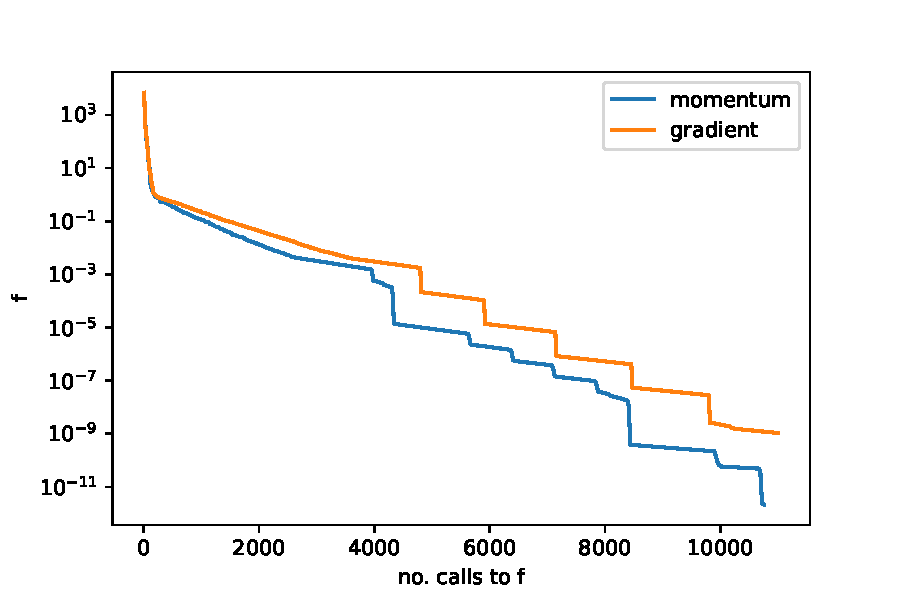
\includegraphics[width=0.7\textwidth]{grad_momentum_quad_10D.pdf}
%\end{center}
%L'accélération par momentum permet un gain de 3 ordres de grandeur dans cette vallée très raide.
%\end{frame}
%%%%%%%%%%%%%%%%%%%%%%%%%%%%%%%%%%%%%%%%%%%%%%%%%%%%%%%%%%%%%%%%%%%
%\begin{frame}
%\frametitle{Gradient accéléré de Nesterov (NAG)}
%Même idée que la direction momentum, mais on anticipe la position du point suivant dans le calcul du gradient
%\cite{nesterov1983method}:
%\begin{equation*}
%s^i = -\bar\alpha \grad f(x^i+\beta (x^i-x^{i-1})) + \beta (x^i -x^{i-1})
%\end{equation*}
%\begin{minipage}[c]{0.5\textwidth}
%Sur le schéma, $\grad f$ tourne vers le haut et le pas est ajusté en conséquence.\
%$s^i$ n'est plus nécessairement une direction de descente.
%\end{minipage}
%\begin{minipage}[c]{0.4\textwidth}
%\begin{center}
%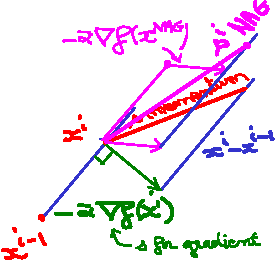
\includegraphics[width=0.9\textwidth]{nag-crop.pdf}
%\end{center}
%\end{minipage}
%\end{frame}
%%%%%%%%%%%%%%%%%%%%%%%%%%%%%%%%%%%%%%%%%%%%%%%%%%%%%%%%%%%%%%%%%%
\begin{frame}
\frametitle{Changement de direction de recherche}
Les méthodes améliorées de gradient modifient légèrement (mais de façon importante) la direction de recherche par rapport à la direction opposée au gradient :
\begin{itemize}
\item Momentum : direction de recherche = direction opposée au gradient déplacée légèrement vers la direction de recherche précédente.
\item Nesterov \cite{nesterov1983method} : direction de recherche = direction momentum avec une anticipation du point du prochain gradient.
\item Adam \cite{kingma2014adam} : état de l’art en apprentissage profond. Méthode de gradient stochastique avec adaptation indépendante de chaque variable basée sur le momentum.
\end{itemize}
\end{frame}
%%%%%%%%%%%%%%%%%%%%%%%%%%%%%%%%%%%%%%%%%%%%%%%%%%%%%%%%%%%%%%%%%%
\begin{frame}
\frametitle{Comparaison des méthodes (1)}
Rosenbrock, $d=2$ : capacité à gérer les ravins courbes
\begin{center}
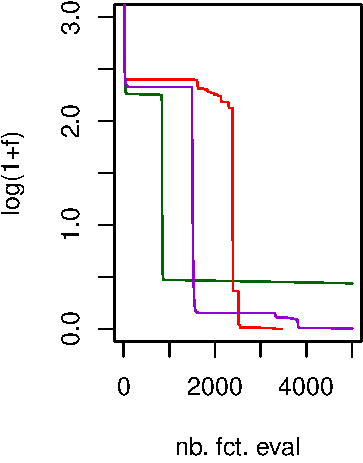
\includegraphics[width=0.4\textwidth]{rosen_comparison-crop.pdf} \
vert=gradient, rouge=momentum, violet=NAG
\end{center}
\end{frame}




%%%%%%%%%%%%%%%%%%%%%%%%%%%%%%%%%%%%%%%%%%%%%%%%%%%%%%%%%%%%%%%%%%%
%\begin{frame}
%\frametitle{Comparaison des méthodes (2)} 
%Tester la vitesse de convergence sur une fonction quadratique, $d=10$, nombre de conditionnement = 100.
%{\small vert=gradient, rouge=momentum, violet=NAG}
%\\\vskip\baselineskip
%\begin{minipage}[c]{0.4\textwidth}
%\begin{center}
%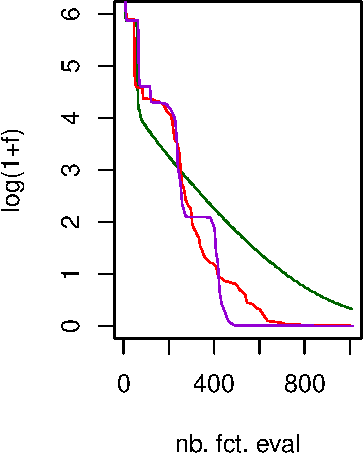
\includegraphics[width=\textwidth]{quadratic_d10_cond100_comparison-crop.pdf} 
%\end{center}
%\end{minipage}
%\hspace{0.6cm}
%\begin{minipage}[c]{0.4\textwidth}
%Conformément à la théorie, la vitesse de convergence de NAG est meilleure que celle du momentum qui est meilleure que celle du gradient.\\
%Notez cependant les plateaux (ou « ondulations ») typiques de NAG et probablement amplifiés par l’approximation par différences finies
%du gradient.
%\end{minipage}
%\end{frame}

% un mot sur la convergence du momentum et de nag : linéaire, seul le coefficient change, ce qui est beaucoup
% comparer les courbes

\subsection{Un mot sur les contraintes}

%%%%%%%%%%%%%%%%%%%%%%%%%%%%%%%%%%%%%%%%%%%%%%%%%%%%%%%%%%%%%%%%%%
\begin{frame}%[allowframebreaks]
\frametitle{Plan du cours} 
\begin{multicols}{2}
\begin{center} \textbf{Introduction à l’optimisation pour l’apprentissage automatique} \end{center}
\tableofcontents[currentsection]
\end{multicols}
\end{frame}

%%%%%%%%%%%%%%%%%%%%%%%%%%%%%%%%%%%%%%%%%%%%%%%%%%%%%%%%%%%%%%%%%%
\begin{frame}
\frametitle{Un mot sur les contraintes} 
\begin{equation*}
\left\{
\begin{array}{l}
\min_{x \in \mathcal S} f(x) \quad,\quad \mathcal S = \Rset[n]\\
\text{tel que } g_i(x) \le 0 \quad , \quad i=1,m
\end{array}
\right.
\end{equation*}
\end{frame}

%%%%%%%%%%%%%%%%%%%%%%%%%%%%%%%%%%%%%%%%%%%%%%%%%%%%%%%%%%%%%%%%%%
\begin{frame}
\frametitle{Contraintes de bornes} 
$\mathcal S$ est un hypercube de $\Rset[n]$, $\mathcal S = [LB,UB] \subset \Rset[n]$.
\vskip\baselineskip
Il peut être décrit par des contraintes, 
$g_{2i-1}(x) \coloneqq LB_i - x_i \le 0$,
$g_{2i}(x) \coloneqq x_i - UB_i \le 0$, $i=1,\ldots,d$
mais ces contraintes sont si simples qu’elles peuvent être directement traitées par projection.\\
\mbox{
\begin{minipage}[c]{0.4\textwidth}
Si $x^i$ est à une borne et que la direction de recherche $d^i$ l’amène en dehors$^a$
de $\mathcal S = [LB,UB]$, 
projeter le vecteur direction de recherche sur la borne active.\\
Exercice : comment coder cela ?
\end{minipage}
\hspace{0.7cm}
\begin{minipage}[c]{0.4\textwidth}
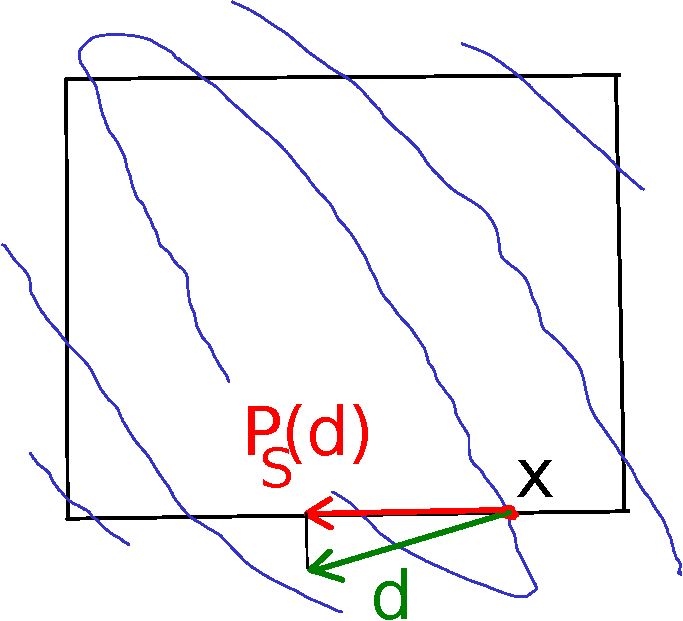
\includegraphics[width=\textwidth]{proj_bound-crop.pdf}
\end{minipage}
}
\\
{$^a$\small Cela peut même arriver pour une fonction convexe dans un $\mathcal S$ convexe, comme le montre le dessin.} 
\end{frame}


%%%%%%%%%%%%%%%%%%%%%%%%%%%%%%%%%%%%%%%%%%%%%%%%%%%%%%%%%%%%%%%%%%
\begin{frame}
\frametitle{Gestion des contraintes par pénalisation (1)} 
\vspace{-0.5cm}
\begin{equation*}
\left\{
\begin{array}{l}
\min_{x \in \mathcal S \in \Rset[d]} f(x) \\
\text{tel que } g(x) \le 0 
\end{array}
\right.
\end{equation*}
\hfill{\scriptsize (notation vectorielle pour les contraintes)}\\
Nous donnons deux techniques pour agréger $f$ et les $g_i$ en une nouvelle fonction objectif 
(à minimiser).
\vskip\baselineskip
\textbf{Fonction de pénalité externe} : pénaliser les points qui ne satisfont pas les contraintes
\begin{equation*}
f_r(x) = f(x) + r \left[\max(0,g(x)) \right]^2 \quad,\quad r>0 
\end{equation*}
\vspace{-0.5cm}
\begin{itemize}
\item{Avantages} : simple, $\grad f_r()$ continue au voisinage de la frontière des contraintes (si $f$ et $g$ le sont)
\item{Inconvénients} : convergence par le domaine infaisable (d’où le nom externe), besoin de trouver un $r$ suffisamment grand pour réduire l’infaisabilité, mais pas trop grand à cause des problèmes numériques (forte courbure au voisinage de la contrainte)
\end{itemize}
\end{frame}

%%%%%%%%%%%%%%%%%%%%%%%%%%%%%%%%%%%%%%%%%%%%%%%%%%%%%%%%%%%%%%%%%%
\begin{frame}
\frametitle{Gestion des contraintes par pénalisation (2)} 
\textbf{Lagrangien} : pour les problèmes sans écart de dualité\footnote{cf. dualité, hors programme de ce cours}, par exemple les problèmes convexes, il existe des multiplicateurs de Lagrange $\lambda^\star$ tels que 
\begin{equation*}
\begin{split}
& x^\star \in \arg \min_{x \in \mathcal S} L(x;\lambda^\star) \\
&\text{où } L(x;\lambda^\star) \coloneqq f(x) + \lambda^\star g(x)
\end{split}
\end{equation*}
Le Lagrangien $L(;\lambda^\star)$ est (en l’absence d’écart de dualité) une fonction de pénalité valide.
\begin{itemize}
\item{Avantages} : la dualité fournit un moyen de calculer $\lambda^\star$, conduit à une solution faisable.
\item{Inconvénients} : estimer $\lambda^\star$ a un coût numérique. 
Pour la plupart des problèmes avec optima locaux, il existe un écart de dualité $\Rightarrow$ on s’appuie alors sur les lagrangiens augmentés$^4$.
\end{itemize}
\end{frame}





%%%%%%%%%%%%%%%%%%%%%%%%%%%%%%%%%%%%%%%%%%%%%%%%%%%%%%%%%%%%%%%%%%
\begin{frame}
\frametitle{Gestion des contraintes par pénalisations (3)} 
Exemple : $f(x)=(x-2)^2$, $g(x)=4-x \leq 0$, $x^*=4$, problème convexe
\vskip\baselineskip
\mbox{
\begin{minipage}[c]{0.35\textwidth}
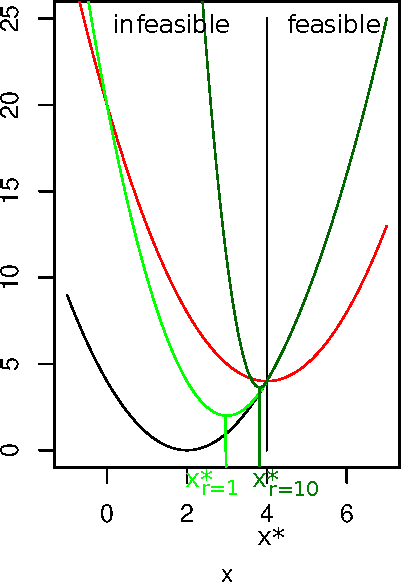
\includegraphics[width=\textwidth]{constraints_methods_annoted-crop.pdf}
\end{minipage}
\hspace{0.5cm}
\begin{minipage}[c]{0.6\textwidth}
$f$ et $g$ en noir, $L(x;\lambda^\star=4)$ en rouge, 
pénalité extérieure $f_r()$ avec $r=1$ et 10 en vert clair et foncé, respectivement.
\vskip\baselineskip
La lagrangienne est ici une pénalité valide. 
\vskip\baselineskip
Quand $r$ augmente, $x_r^\star \rightarrow x^\star$ mais la courbure de $f_r()$ augmente.
\end{minipage}
}
\end{frame}

%%%%%%%%%%%%%%%%%%%%%%%%%%%%%%%%%%%%%%%%%%%%%%%%%%%%%%%%%%%%%%%%%%
\begin{frame}
\frametitle{Commentaires sur les algorithmes de descente basés sur le gradient} 
\begin{minipage}[c]{0.5\textwidth}
Utilisation sur des fonctions non différentiables : théoriquement peut converger vers un point qui n’est pas un minimum même pour des fonctions convexes (par ex. si un itéré se trouve à un point anguleux). Cela arrive rarement en pratique. 
Essayez la fonction $f(x) = \sum_{i=1}^n |x_i|$ (``norme L1'') avec le code. 
\end{minipage}
\begin{minipage}[c]{0.4\textwidth}
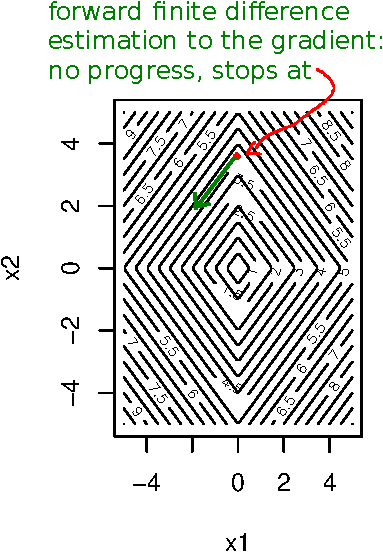
\includegraphics[width=\textwidth]{L1norm_contour-premconv-crop.pdf} 
\end{minipage}
\\
Principal défaut : peut rester bloqué dans des minima locaux.
\end{frame}

\subsection{Rendre la méthode plus globale : redémarrages}

%%%%%%%%%%%%%%%%%%%%%%%%%%%%%%%%%%%%%%%%%%%%%%%%%%%%%%%%%%%%%%%%%%
\begin{frame}
\frametitle{Redémarrages des recherches locales} 
Principe simple : redémarrer les recherches par descente à partir de points initiaux choisis aléatoirement.\\
Utiliser l’aléa pour rendre les recherches déterministes par descente plus robustes.\\
Un compromis entre 2 extrêmes : local vs global, recherche linéaire vs recherche volumique, spécifique (aux fonctions unimodales différentiables) vs sans hypothèse, efficace vs très lent.\\
Implémentation simpliste 
%(cf. code fourni) \\ \hspace{5cm} 
au coût multiplié par \texttt{nb\_restarts} :
\vspace{-0.4cm}
\begin{center}
\begin{minipage}[t]{\textwidth}
\begin{algorithmic}
\REQUIRE \texttt{budget}, \texttt{nb\_restarts}
\FOR {\texttt{i in 1} \TO \texttt{nb\_restarts} }
\STATE \texttt{xinit <- runif(n=d,min=LB,max=UB)}
\STATE \texttt{res<-gradient\_descent(xinit,budget=budget/nb\_restarts)}
\STATE {mettre à jour les résultats globaux de la recherche}
\ENDFOR
\end{algorithmic}
\end{minipage}
\end{center}
\end{frame}

%%%%%%%%%%%%%%%%%%%%%%%%%%%%%%%%%%%%%%%%%%%%%%%%%%%%%%%%%%%%%%%%%%
\begin{frame}
\frametitle{Redémarrages des recherches locales : exemple} 
Exécution du fichier \texttt{restarted\_descent}. \\
\texttt{fun <- rastrigin, d <- 2, budget <- 1000, nb\_restart <- 10} :
\begin{center}
\mbox{
\begin{minipage}[t]{0.4\textwidth}
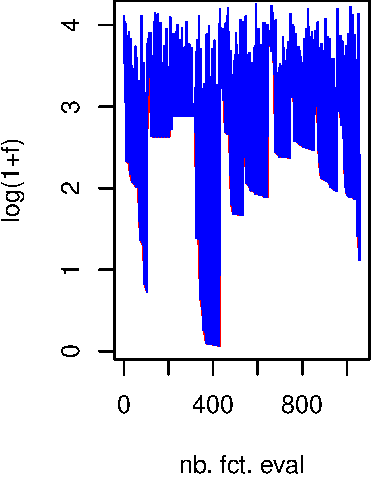
\includegraphics[width=\textwidth]{rastrigin_budget1000_restart10_f-crop.pdf}
\end{minipage}
\vspace{0.7cm}
\begin{minipage}[t]{0.4\textwidth}
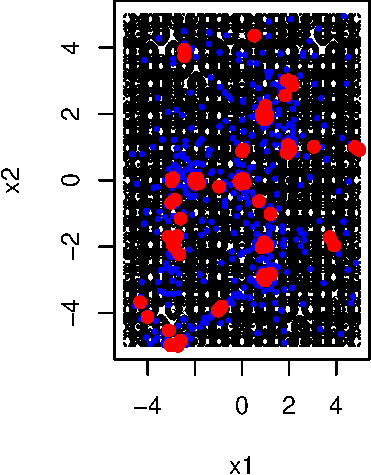
\includegraphics[width=\textwidth]{rastrigin_budget1000_restart10_x-crop.pdf}
\end{minipage}
}
\end{center}
\end{frame}


\section{Application aux réseaux de neurones}

%%%%%%%%%%%%%%%%%%%%%%%%%%%%%%%%%%%%%%%%%%%%%%%%%%%%%%%%%%%%%%%%%%
\begin{frame}%[allowframebreaks]
\frametitle{Application aux réseaux de neurones} 
\begin{center}
Les applications pratiques sont disponibles via le notebook \texttt{project} sur github,\\
cf. \url{https://github.com/ML-for-B-E/Optimisation/notebook/project.ipynb}
\end{center}
\end{frame}

\section*{Conclusions}

%%%%%%%%%%%%%%%%%%%%%%%%%%%%%%%%%%%%%%%%%%%%%%%%%%%%%%%%%%%%%%%%%
\begin{frame}
\frametitle{Conclusions}
\begin{itemize}
\item L’optimisation numérique est une technique fondamentale pour la prise de décision quantitative, la modélisation statistique, l’apprentissage automatique, \ldots
\item L’engouement pour l’apprentissage automatique a conduit à de très nombreux algorithmes d’optimisation que nous n’avons pas abordés dans ce cours introductif : voir par exemple \cite{sun2019survey,sra2012optimization}. 
\item Egalement non traitée mais en émergence : l’optimisation bayésienne pour le réglage des hyperparamètres (constantes de régularisation, nombre de couches de réseaux de neurones, types de neurones, paramètres des algorithmes basés sur le gradient) \cite{snoek2012practical}.
\end{itemize}
\end{frame}

%%%%%%%%%%%%%%%%%%%%%%%%%%%%%%%%%%%%%%%%%%%%%%%%%%%%%%%%%%%%%%%%%
\begin{frame}
\frametitle{Références bibliographiques pour le cours}
{\small
Ce cours est basé sur
\begin{itemize}
\item \cite{ravikumar17} : une présentation détaillée et à jour des principaux algorithmes d’optimisation convexe pour l’apprentissage automatique (niveau fin licence, bac +3)
\item \cite{minoux2008programmation} : un manuel classique d’optimisation, écrit avant la mode ML mais toujours utile (niveau fin licence / bac+3)
\item \cite{bishop2006pattern} : un ouvrage de référence en apprentissage automatique avec quelques pages sur l’optimisation (niveau fin licence / bac+3)
\item \cite{schmidt2007fast} : techniques de régularisation L1 (article de recherche)
\item \cite{sun2019optimization} : revue des méthodes d’optimisation et bonnes pratiques pour le réglage des réseaux de neurones.
\end{itemize}
Le contenu de ces références a été simplifié pour ce cours.
} % fin petit texte
\end{frame}

\section{Bibliographie}

%=======================================================================================
\begin{frame}[allowframebreaks]
\frametitle{Références}
\scriptsize
%\vspace{-1.cm}
%\setbeamertemplate{bibliography item}{[\theenumiv]} % pour avoir des numéros dans la biblio avec beamer
%   \bibliographystyle{plain}
   \bibliographystyle{apalike}
   \bibliography{biblio}
\end{frame}

\end{document}
